%_____________________________________________________________________________
%=============================================================================
% main.tex v6 (10-11-2013) \ldots dibuat oleh Lionov - Informatika FTIS UNPAR
% 
% Ini adalah file utama (main.tex), berisi perintah-perintah yang khusus 
% dibuat untuk template ini
%
% 			JANGAN MENGUBAH APAPUN DI DALAM FILE INI,
%			KECUALI ANDA TAHU APA YANG ANDA LAKUKAN !!!
%
% Jika ada tambahan perintah, dapat anda tuliskan di tempat yang telah disediakan 
% di baris 295 pada file ini
% Jika daftar tabel tidak digunakan, anda harus menghapus (beri komentar) secara
% manual di baris 470
%
% Bug, kritik, saran: silahkan kirimkan via email ke lionov@unpar.ac.id
%
% Perubahan pada versi 6 (10-11-2013):
%	- perbaikan pada abstract dengan paragraf lebih dari satu: perbaikan vertical spacing
%	- perbaikan pada tampilan bab dan lampiran: tidak perlu menuliskan apapun untuk 
%	  menampilkan semuanya (di data.tex) atau -1 jika tidak ada lampiran
%	- halaman bernomor genap untuk halaman romawi sudah dimunculkan
%	- Kurikulum 2013 : perubahan nama buku skripsi 
%
% Perubahan dari versi sebelumnya :
%	versi 5 (21-10-2012)
%	- halaman terakhir setiap bab tidak ada headernya jika kosong
%	versi 4 (06-08-2012)
% 	- penggabungan main.tex, depan.tex dan setup.tex menjadi main.tex
% 	- menambahkan keterangan di lampiran untuk kode program 
% 	- ukuran font dapat diubah langsung di tiap lampiran
% 	versi 3 (09-07-2012): 
%	- Tidak ada di file ini
% 	versi 2 :
% 	- "Daftar Referensi" tidak perlu diubah secara manual (tidak perlu mengubah file bahasai.ldf)
% 	- Bahasa Indonesia dari abstract adalah abstrak (secara otomatis), bukan ringkasan
% 	- Spasi pada buku dokumen final adalah onehalfspacing
%
% to do : - hilangkan secara otomatis daftar tabel/gambar jika tidak digunakan
%         - (IT) aturan penulisan algoritma untuk IT (pakai algo.sty ?)
%=============================================================================

%=============================================================================
% setup.tex v2 (08-07-2012)
% Perubahan pada versi 2:
% - Menambahkan perintah untuk judulINA dan judulENG
% - Menghapus \usepackage{microtype}, yang pada beberapa kasus menjadi masalah
%=============================================================================
% depan.tex v2 (09-07-2012)
% Perubahan pada versi 2:
% - Menambahkan halaman depan dalam bahasa inggris
%=============================================================================

%setup.tex
\documentclass[11pt,a4paper,twoside,openright,notitlepage]{report} 

\usepackage[bahasa]{babel} %bahasa indonesia
\usepackage[T1]{fontenc}  %encoding
% \usepackage{mathptmx}
% \usepackage{venturisold}
% \usepackage{helvet}
% \usepackage{fouriernc} 
\usepackage{abstract} %manipulasi abstract
\usepackage{chappg} % format daftar isi 
\usepackage{color} %warna
\usepackage{etoolbox} %untuk programming if-then
\usepackage{fancyhdr} %format header & footer
\usepackage{float} %penempatan gambar di tempat yg seharusnya
\usepackage[inner=2.5cm,outer=2cm,top=2.5cm,bottom=2.5cm]{geometry} %margin
\usepackage{graphicx} %gambar
\usepackage{listings} %source code
\usepackage{lscape} %landscape untuk source code
\usepackage{multicol} %multiple column
\usepackage{ifthen} % if then
\usepackage[pagewise]{lineno} %line numbering
\usepackage{lipsum} % untuk testing
\usepackage{titlesec} %judul header
\usepackage{tocbibind} %daftar isi, gambar, tabel dll
\usepackage{tocloft} % format daftar isi 
\usepackage{setspace} %line spacing
\usepackage{xstring} %manipulasi string
\usepackage[plainpages=false,pdfpagelabels,unicode]{hyperref} %\autoref, \phantomsection & link 

\usepackage{emptypage}

\let\abstractname\Abstrak

\titleformat{\chapter}[display] {\Large\bfseries\centering}{\MakeUppercase{\chaptertitlename} \thechapter}{15pt}{\Large\MakeUppercase}

\renewcommand{\cftchapfont}{\scshape \bfseries}

\renewcommand{\cfttoctitlefont}{\hfill\Large\bfseries\MakeUppercase}
\renewcommand{\cftaftertoctitle}{\hfill}
\renewcommand{\cftloftitlefont}{\hfill\Large\bfseries\MakeUppercase}
\renewcommand{\cftafterloftitle}{\hfill}
\renewcommand{\cftlottitlefont}{\hfill\Large\bfseries\MakeUppercase}
\renewcommand{\cftafterlottitle}{\hfill}

% Tidak perlu ada kata "Bab", "Gambar" atau "Tabel" di daftar 
% \renewcommand{\cftchappresnum}{{\bf \scshape Bab} } 
% \renewcommand{\cftchapnumwidth}{1.5cm}
% \renewcommand{\cftfigpresnum}{{Gambar\ }} 
% \renewcommand{\cftfignumwidth}{2.5cm}
% \renewcommand{\cfttabpresnum}{{Tabel\ }} 
% \renewcommand{\cfttabnumwidth}{2cm}

\newcommand{\apptoc}{
	% Hapus kata "Lampiran" dari daftar isi
	%\addtocontents{toc}{\protect\renewcommand{\protect\cftchappresnum}{\bf \scshape Lampiran\  }}%
	%\addtocontents{toc}{\protect\renewcommand{\protect\cftchapnumwidth}{2.75cm}}
	\addtocontents{toc}{\protect\renewcommand{\protect\cftchappresnum}{\bf \scshape}}%	

}

\newcommand{\vnama}{Jane Doe}
\newcommand{\vlnama}{John Doe}
\newcommand{\vnpm}{1992700001}
\newcommand{\vprodiINA}{SAINS}
\newcommand{\vprodiENG}{SCIENCE}
\newcommand{\vstaINA}{UJIAN}
\newcommand{\vstaENG}{EXAM}
%\newcommand{\vjudul}{Judul Skripsi/Tugas Akhir}
\newcommand{\vpembu}{Plato}
\newcommand{\vpembs}{Euclid}
\newcommand{\vpengi}{Plato}
\newcommand{\vpengii}{Euclid}
\newcommand{\vtanggal}{1}
\newcommand{\vbulan}{Januari}
\newcommand{\vtahun}{1970}
\newcommand{\vmode}{final}
\newcommand{\vspacing}{double}
\newcommand{\vlineno}{yes}
\newcommand{\vkunciina}{Skripsi, Tugas Akhir}
\newcommand{\vkuncieng}{Undergraduate Thesis, Final Project}
\newcommand{\vkajur}{Jack Doe}
\newcommand{\vkajurmat}{Jack Doe}
\newcommand{\vkajurfis}{Jack Doe}
\newcommand{\vkajurtif}{Jack Doe}

\newcommand{\namanpm}[2]{
	\renewcommand{\vnama}{\uppercase{#1}} \renewcommand{\vlnama}{#1} \hypersetup{pdfauthor={#2 - #1}}
	\renewcommand{\vnpm}{#2} \hypersetup{pdfcreator={#2}} \StrChar{\vnpm}{6}[\vprodiN]
	\ifdefstring{\vprodiN}{1}{
		\renewcommand{\vprodiINA}{MATEMATIKA} \renewcommand{\vprodiENG}{MATHEMATICS} 
		\renewcommand{\vstaINA}{SKRIPSI} \renewcommand{\vstaENG}{FINAL PROJECT} \renewcommand{\vkajur}{\vkajurmat}}{}
	\ifdefstring{\vprodiN}{2}{
		\renewcommand{\vprodiINA}{FISIKA} \renewcommand{\vprodiENG}{PHYSICS} 
		\renewcommand{\vstaINA}{TUGAS AKHIR} \renewcommand{\vstaENG}{FINAL PROJECT} \renewcommand{\vkajur}{\vkajurfis}}{}
	\ifdefstring{\vprodiN}{3}{
		\renewcommand{\vprodiINA}{TEKNIK INFORMATIKA} \renewcommand{\vprodiENG}{INFORMATICS} 
		\renewcommand{\vstaINA}{SKRIPSI} \renewcommand{\vstaENG}{UNDERGRADUATE THESIS} \renewcommand{\vkajur}{\vkajurtif}}{}}

%\newcommand{\judul}[1]{\renewcommand{\vjudul}{\uppercase{#1}}\hypersetup{pdftitle={#1}, pdfsubject={#1}}}
\newcommand{\pembimbing}[2]{\renewcommand{\vpembu}{#1}\renewcommand{\vpembs}{#2}}
\newcommand{\penguji}[2]{\renewcommand{\vpengi}{#1}\renewcommand{\vpengii}{#2}}
\newcommand{\kajur}[3]{\renewcommand{\vkajurmat}{#1}\renewcommand{\vkajurfis}{#2}\renewcommand{\vkajurtif}{#3}}
\newcommand{\tanggal}[3]{\renewcommand{\vtanggal}{#1}\renewcommand{\vtahun}{#3}
	\newcommand{\vcbulan}{#2}
	\ifdefstring{\vcbulan}{1}{\renewcommand{\vbulan}{Januari}}{}
	\ifdefstring{\vcbulan}{2}{\renewcommand{\vbulan}{Februari}}{}
	\ifdefstring{\vcbulan}{3}{\renewcommand{\vbulan}{Maret}}{}
	\ifdefstring{\vcbulan}{4}{\renewcommand{\vbulan}{April}}{}
	\ifdefstring{\vcbulan}{5}{\renewcommand{\vbulan}{Mei}}{}
	\ifdefstring{\vcbulan}{6}{\renewcommand{\vbulan}{Juni}}{}
	\ifdefstring{\vcbulan}{7}{\renewcommand{\vbulan}{Juli}}{}
	\ifdefstring{\vcbulan}{8}{\renewcommand{\vbulan}{Agustus}}{}
	\ifdefstring{\vcbulan}{9}{\renewcommand{\vbulan}{September}}{}
	\ifdefstring{\vcbulan}{10}{\renewcommand{\vbulan}{Oktober}}{}
	\ifdefstring{\vcbulan}{11}{\renewcommand{\vbulan}{November}}{}
	\ifdefstring{\vcbulan}{12}{\renewcommand{\vbulan}{Desember}}{}	
}

\newcommand{\judulINA}[1]{\newcommand{\vjudulINA}{\uppercase{#1}}\hypersetup{pdftitle={#1},pdfsubject={#1}}}
\newcommand{\judulENG}[1]{\newcommand{\vjudulENG}{\uppercase{#1}}\hypersetup{pdftitle={#1},pdfsubject={#1}}}
\newcommand{\abstrakINA}[1]{\newcommand{\vabstrakina}{#1}}
\newcommand{\abstrakENG}[1]{\newcommand{\vabstrakeng}{#1}}
\newcommand{\kunciINA}[1]{\renewcommand{\vkunciina}{#1} \hypersetup{pdfkeywords={#1}}}
\newcommand{\kunciENG}[1]{\renewcommand{\vkuncieng}{#1}}
\newcommand{\untuk}[1]{\newcommand{\vuntuk}{#1}}
\newcommand{\prakata}[1]{\newcommand{\vprakata}{#1}}
\newcommand{\mode}[1]{\renewcommand{\vmode}{#1}}
\newcommand{\linespacing}[1]{\renewcommand{\vspacing}{#1}}
\newcommand{\linenumber}[1]{\renewcommand{\vlineno}{#1}}

\newcommand{\bab}[1]{\newcommand{\vbab}{#1}}
\newcommand{\lampiran}[1]{\renewcommand{\vlmp}{#1}}

\newcommand{\vpilbab}{0}
\newcommand{\vbaba}{0}\newcommand{\vbabb}{0}\newcommand{\vbabc}{0}
\newcommand{\vbabd}{0}\newcommand{\vbabe}{0}\newcommand{\vbabf}{0}
\newcommand{\vbabg}{0}\newcommand{\vbabh}{0}\newcommand{\vbabi}{0}
\newcommand{\vpillmp}{0}
\newcommand{\vlmpa}{0}\newcommand{\vlmpb}{0}\newcommand{\vlmpc}{0}
\newcommand{\vlmpd}{0}\newcommand{\vlmpe}{0}\newcommand{\vlmpf}{0}
\newcommand{\vlmpg}{0}\newcommand{\vlmph}{0}\newcommand{\vlmpi}{0}
\newcommand{\vlmp}{x}

%	\ifdefempty{#1}{\bab{1,2,3,4,5,6,7,8,9} \tampilbab{\vbab}}{
\newcommand{\tampilbab}[1]{
	\ifdefempty{#1}{
		\renewcommand{\vbaba}{1}\renewcommand{\vbabb}{1}\renewcommand{\vbabc}{1}
		\renewcommand{\vbabd}{1}\renewcommand{\vbabe}{1}\renewcommand{\vbabf}{1}
		\renewcommand{\vbabg}{1}\renewcommand{\vbabh}{1}\renewcommand{\vbabi}{1}}{
	\renewcommand{\do}[1]{
		\renewcommand{\vpilbab}{##1}
		\ifdefstring{\vpilbab}{1}{\renewcommand{\vbaba}{1}}{}
		\ifdefstring{\vpilbab}{2}{\renewcommand{\vbabb}{1}}{}
		\ifdefstring{\vpilbab}{3}{\renewcommand{\vbabc}{1}}{}
		\ifdefstring{\vpilbab}{4}{\renewcommand{\vbabd}{1}}{}
		\ifdefstring{\vpilbab}{5}{\renewcommand{\vbabe}{1}}{}
		\ifdefstring{\vpilbab}{6}{\renewcommand{\vbabf}{1}}{}
		\ifdefstring{\vpilbab}{7}{\renewcommand{\vbabg}{1}}{}
		\ifdefstring{\vpilbab}{8}{\renewcommand{\vbabh}{1}}{}
		\ifdefstring{\vpilbab}{9}{\renewcommand{\vbabi}{1}}{}
	}
	\expandafter\docsvlist\expandafter{#1}
	}
}

\newcommand{\tampillmp}[1]{
	\ifdefempty{#1}{
		\renewcommand{\vlmpa}{1}\renewcommand{\vlmpb}{1}\renewcommand{\vlmpc}{1}
		\renewcommand{\vlmpd}{1}\renewcommand{\vlmpe}{1}\renewcommand{\vlmpf}{1}
		\renewcommand{\vlmpg}{1}\renewcommand{\vlmph}{1}\renewcommand{\vlmpi}{1}}{
	\ifdefstring{#1}{-1}{ }{
		\renewcommand{\do}[1]{ 
			\renewcommand{\vpillmp}{##1}
			\ifdefstring{\vpillmp}{A}{\renewcommand{\vlmpa}{1}}{}
			\ifdefstring{\vpillmp}{B}{\renewcommand{\vlmpb}{1}}{}
			\ifdefstring{\vpillmp}{C}{\renewcommand{\vlmpc}{1}}{}
			\ifdefstring{\vpillmp}{D}{\renewcommand{\vlmpd}{1}}{}
			\ifdefstring{\vpillmp}{E}{\renewcommand{\vlmpe}{1}}{}
			\ifdefstring{\vpillmp}{F}{\renewcommand{\vlmpf}{1}}{}
			\ifdefstring{\vpillmp}{G}{\renewcommand{\vlmpg}{1}}{}
			\ifdefstring{\vpillmp}{H}{\renewcommand{\vlmph}{1}}{}
			\ifdefstring{\vpillmp}{I}{\renewcommand{\vlmpi}{1}}{}}
		}
	\expandafter\docsvlist\expandafter{#1}
	}
}

\newcommand{\appspacing}{
	\ifdefstring{\vspacing}{single}{\singlespacing}{}
	\ifdefstring{\vspacing}{onehalf}{\onehalfspacing}{}
	\ifdefstring{\vspacing}{double}{\doublespacing}{}
	\ifdefstring{\vmode}{final}{\onehalfspacing}{}
}

\newcommand{\appline}{
	\ifdefstring{\vmode}{final}{\renewcommand{\vlineno}{no}}{}
	\ifdefstring{\vlineno}{yes}{\linenumbers \def\linenumberfont{\normalfont\tiny\sffamily}}{}
	\ifdefstring{\vlineno}{no}{\lstset{numbers=left, stepnumber=1, numbersep=5pt}}{}
	
}

\newcommand{\appmargin}{
	\ifdefstring{\vmode}{final}{}{\newgeometry{inner=3cm,outer=2.75cm,top=2cm,bottom=2cm}}
}

\renewcommand{\abstractnamefont}{\bf \MakeUppercase}

\makeatletter
\def\headrule{{%
  \if@fancyplain\let\headrulewidth\plainheadrulewidth\fi
  \hrule\@height\footrulewidth\@width\headwidth\vskip2pt%
  \hrule\@height\headrulewidth\@width\headwidth\vskip-\headrulewidth\vskip-4pt
}}
\def\footrule{}

\def\cleardoublepage{
	\clearpage
	\if@twoside \ifodd\c@page
	\else
		\hbox{}
		\vspace{\fill}
		\thispagestyle{empty}
		\newpage
	\if@twocolumn\hbox{}\newpage\fi\fi\fi}
\makeatother

\renewcommand{\headrulewidth}{1.25pt}
\renewcommand{\footrulewidth}{0.25pt}

\setlength{\headheight}{15pt}
\fancyhead[LE,RO]{\thepage}
\fancyhead[RE]{\small{\textsc{\nouppercase{\leftmark}}}}
\fancyhead[LO]{\small{\textsc{\nouppercase{\rightmark}}}}
\fancyfoot{}

\hypersetup{unicode=true,colorlinks=true,linkcolor=blue,citecolor=green,filecolor=magenta, urlcolor=cyan}

\lstset{basicstyle=\tiny, commentstyle=\color{blue}}
\lstset{frame=leftline, tabsize=4, breaklines=true}

%=============================================================================

%tambahkan perintah yang anda butuhkan di sini :

%=============================================================================
%end setup.tex

%_____________________________________________________________________________
%=============================================================================
% data.tex v6 (13-04-2015) \ldots dibuat oleh Lionov - Informatika FTIS UNPAR
%
% Perubahan pada versi 6 (13-04-2015)
% - Perubahan untuk data-data ``template" menjadi lebih generik dan menggunakan
%	tanda << dan >>
%
% Perubahan pada versi sebelumnya
% 	versi 5 (10-11-2013)
% 	- Perbaikan pada memasukkan bab : tidak perlu menuliskan apapun untuk 
%	  memasukkan seluruh bab (bagian V)
% 	- Perbaikan pada memasukkan lampiran : tidak perlu menuliskan apapun untuk
%	  memasukkan seluruh lampiran atau -1 jika tidak memasukkan apapun
%	versi 4 (21-10-2012)
%	- Data dosen dipindah ke dosen.tex agar jika ada perubahan/update data dosen
%   mahasiswa tidak perlu mengubah data.tex
%	- Perubahan pada keterangan dosen	
% 	versi 3 (06-08-2012)
% 	- Perubahan pada beberapa keterangan 
% 	versi 2 (09-07-2012):
% 	- Menambahkan data judul dalam bahasa inggris
% 	- Membuat bagian khusus untuk judul (bagian VIII)
% 	- Perbaikan pada gelar dosen
%_____________________________________________________________________________
%=============================================================================
% 								BAGIAN -
%=============================================================================
% Ini adalah file data (data.tex)
% Masukkan ke dalam file ini, data-data yang diperlukan oleh template ini
% Cara memasukkan data dijelaskan di setiap bagian
% Data yang WAJIB dan HARUS diisi dengan baik dan benar adalah SELURUHNYA !!
% Hilangkan tanda << dan >> jika anda menemukannya
%=============================================================================
%_____________________________________________________________________________
%=============================================================================
% 								BAGIAN I
%=============================================================================
% Tambahkan package2 lain yang anda butuhkan di sini
%=============================================================================
\usepackage{booktabs}
\usepackage[table]{xcolor}
\usepackage{longtable}
\usepackage{amsmath}
%=============================================================================

%_____________________________________________________________________________
%=============================================================================
% 								BAGIAN II
%=============================================================================
% Mode dokumen: menetukan halaman depan dari dokumen, apakah harus mengandung 
% prakata/pernyataan/abstrak dll (termasuk daftar gambar/tabel/isi) ?
% - kosong : tidak ada halaman depan sama sekali (untuk dokumen yang 
%            dipergunakan pada proses bimbingan)
% - cover : cover saja tanpa daftar isi, gambar dan tabel
% - sidang : cover, daftar isi, gambar, tabel (IT: UTS-UAS Seminar 
%			 dan UTS TA)
% - sidang_akhir : mode sidang + abstrak + abstract
% - final : seluruh halaman awal dokumen (untuk cetak final)
% Jika tidak ingin mencetak daftar tabel/gambar (misalkan karena tidak ada 
% isinya), edit manual di baris 439 dan 440 pada file main.tex
%=============================================================================
% \mode{kosong}
% \mode{cover}
% \mode{sidang}
%\mode{sidang_akhir}
\mode{final} 
%=============================================================================

%_____________________________________________________________________________
%=============================================================================
% 								BAGIAN III
%=============================================================================
% Line numbering: penomoran setiap baris, otomatis di-reset setiap berganti
% halaman
% - yes: setiap baris diberi nomor
% - no : baris tidak diberi nomor, otomatis untuk mode final
%=============================================================================
\linenumber{yes}
%=============================================================================

%_____________________________________________________________________________
%=============================================================================
% 								BAGIAN IV
%=============================================================================
% Linespacing: jarak antara baris 
% - single: opsi yang disediakan untuk bimbingan, jika pembimbing tidak
%            keberatan (untuk menghemat kertas)
% - onehalf: default dan wajib (dan otomatis) jika ingin mencetak dokumen
%            final/untuk sidang.
% - double : jarak yang lebih lebar lagi, jika pembimbing berniat memberi 
%            catatan yg banyak di antara baris (dianjurkan untuk bimbingan)
%=============================================================================
\linespacing{single}
% \linespacing{onehalf}
%\linespacing{double}
%=============================================================================

%_____________________________________________________________________________
%=============================================================================
% 								BAGIAN V
%=============================================================================
% Bab yang akan dicetak: isi dengan angka 1,2,3 s.d 9, sehingga bisa digunakan
% untuk mencetak hanya 1 atau beberapa bab saja
% Jika lebih dari 1 bab, pisahkan dengan ',', bab akan dicetak terurut sesuai 
% urutan bab.
% Untuk mencetak seluruh bab, kosongkan parameter (i.e. \bab{ })  
% Catatan: Jika ingin menambahkan bab ke-10 dan seterusnya, harus dilakukan 
% secara manual
%=============================================================================
\bab{ }
%=============================================================================

%_____________________________________________________________________________
%=============================================================================
% 								BAGIAN VI
%=============================================================================
% Lampiran yang akan dicetak: isi dengan huruf A,B,C s.d I, sehingga bisa 
% digunakan untuk mencetak hanya 1 atau beberapa lampiran saja
% Jika lebih dari 1 lampiran, pisahkan dengan ',', lampiran akan dicetak 
% terurut sesuai urutan lampiran
% Jika tidak ingin mencetak lampiran apapun, isi dengan -1 (i.e. \lampiran{-1})
% Untuk mencetak seluruh mapiran, kosongkan parameter (i.e. \lampiran{ })  
% Catatan: Jika ingin menambahkan lampiran ke-J dan seterusnya, harus 
% dilakukan secara manual
%=============================================================================
\lampiran{ }
%=============================================================================

%_____________________________________________________________________________
%=============================================================================
% 								BAGIAN VII
%=============================================================================
% Data diri dan skripsi/tugas akhir
% - namanpm: Nama dan NPM anda, penggunaan huruf besar untuk nama harus benar
%			 dan gunakan 10 digit npm UNPAR, PASTIKAN BAHWA BENAR !!!
%			 (e.g. \namanpm{Jane Doe}{1992710001}
% - judul : Dalam bahasa Indonesia, perhatikan penggunaan huruf besar, judul
%			tidak menggunakan huruf besar seluruhnya !!! 
% - tanggal : isi dengan {tangga}{bulan}{tahun} dalam angka numerik, jangan 
%			  menuliskan kata (e.g. AGUSTUS) dalam isian bulan
%			  Tanggal ini adalah tanggal dimana anda akan melaksanakan sidang 
%			  ujian akhir skripsi/tugas akhir
% - pembimbing: isi dengan pembimbing anda, lihat daftar dosen di file dosen.tex
%				jika pembimbing hanya 1, kosongkan parameter kedua 
%				(e.g. \pembimbing{\JND}{  } ) , \JND adalah kode dosen
% - penguji : isi dengan para penguji anda, lihat daftar dosen di file dosen.tex
%				(e.g. \penguji{\JHD}{\JCD} ) , \JND dan \JCD adalah kode dosen
%
%=============================================================================
\namanpm{<<Nama Lengkap>>}{<<10 digit NPM UNPAR>>}	%hilangkan tanda << & >>
\tanggal{<<tanggal>>}{<<bulan>>}{<<tahun>>}			%hilangkan tanda << & >>
\pembimbing{<<pembimbing utama/1>>}{<<pembimbing pendamping/2>>}     
%Lihat singkatan pembimbing anda di file dosen.tex, hilangkan tanda << & >>
\penguji{<<penguji 1>>}{<<penguji 2>>} 		
%Lihat singkatan penguji anda di file dosen.tex, hilangkan tanda << & >>
%=============================================================================

%_____________________________________________________________________________
%=============================================================================
% 								BAGIAN VIII
%=============================================================================
% Judul dan title : judul bhs indonesia dan inggris
% - judulINA: judul dalam bahasa indonesia
% - judulENG: title in english
% PERHATIAN: - langsung mulai setelah '{' awal, jangan mulai menulis di baris 
%			   bawahnya
%			 - Gunakan \texorpdfstring{\\}{} untuk pindah ke baris baru
%			 - Judul TIDAK ditulis dengan menggunakan huruf besar seluruhnya !!
%			 - Gunakan perintah \texorpdfstring{\\}{} untuk baris baru
%=============================================================================

\judulINA{<<Judul Bahasa Indonesia>>}

\judulENG{<<Judul Bahasa Inggris>>}

%_____________________________________________________________________________
%=============================================================================
% 								BAGIAN IX
%=============================================================================
% Abstrak dan abstract : abstrak bhs indonesia dan inggris
% - abstrakINA: abstrak bahasa indonesia
% - abstrakENG: abstract in english
% PERHATIAN: langsung mulai setelah '{' awal, jangan mulai menulis di baris 
%			 bawahnya
%=============================================================================

\abstrakINA{<<Tuliskan abstrak anda di sini, dalam bahasa Indonesia>> \lipsum[5]}

\abstrakENG{<<Tuliskan abstrak anda di sini, dalam bahasa Inggris>> \lipsum[5]} 

%=============================================================================

%_____________________________________________________________________________
%=============================================================================
% 								BAGIAN X
%=============================================================================
% Kata-kata kunci dan keywords : diletakkan di bawah abstrak (ina dan eng)
% - kunciINA: kata-kata kunci dalam bahasa indonesia
% - kunciENG: keywords in english
%=============================================================================
\kunciINA{<<Tuliskan di sini kata-kata kunci yang anda gunakan, dalam bahasa Indonesia>>}

\kunciENG{<<Tuliskan di sini kata-kata kunci yang anda gunakan, dalam bahasa Inggris>>}
%=============================================================================

%_____________________________________________________________________________
%=============================================================================
% 								BAGIAN XI
%=============================================================================
% Persembahan : kepada siapa anda mempersembahkan skripsi ini ...
%=============================================================================
\untuk{<<kepada siapa anda mempersembahkan skripsi ini\ldots?>>}
%=============================================================================

%_____________________________________________________________________________
%=============================================================================
% 								BAGIAN XII
%=============================================================================
% Kata Pengantar: tempat anda menuliskan kata pengantar dan ucapan terima 
% kasih kepada yang telah membantu anda bla bla bla ....  
%=============================================================================
\prakata{\lipsum[3]}
%=============================================================================

%_____________________________________________________________________________
%=============================================================================
% 								BAGIAN XIII
%=============================================================================
% Tambahkan hyphen (pemenggalan kata) yang anda butuhkan di sini 
%=============================================================================
\hyphenation{ma-te-ma-ti-ka}
\hyphenation{fi-si-ka}
\hyphenation{tek-nik}
\hyphenation{in-for-ma-ti-ka}
%=============================================================================


%=============================================================================

%_____________________________________________________________________________
%=============================================================================
% dosen.tex v6 (19-08-2016) \ldots dibuat oleh Lionov - Informatika FTIS UNPAR
%
% Perubahan pada versi 6 (19-08-2016)
% 	- Penambahan dosen (Farica, Claudio).
%	- Penghapusan dosen (Oerip)
% 	- Perubahan singkatan untuk dosen Informatika sesuai ketentuan prodi
%	- Perbaikan "catatan untuk mhs teknik informatika"
%
% Perubahan pada versi sebelumnya dapat dilihat di bagian akhir file ini
%_____________________________________________________________________________
%=============================================================================

%=============================================================================
% Data dosen dan kajur FTIS - JANGAN MENGUBAH APAPUN DI BAGIAN INI, KECUALI
% untuk mengubah kajur (jika kajur telah berganti orang) atau menambahkan 
% pembimbing anda yang tidak/belum tercantum pada daftar ini atau 
% memperbaiki penulisan gelar jika penguji anda meminta
% perintah: \kajur{1}{2}{3} 1: Matematika 2: Fisika 3: Teknik Informatika
%=============================================================================
% CATATAN UNTUK MAHASISWA TEKNIK INFORMATIKA :
% dosen yang ditandai * :
% - jika menjadi pembimbing : harus diganti, penggantinya mengikuti petunjuk
% 	dari koordinator Skripsi !
% - jika menjadi penguji: tidak diganti, tetapi hapus komentar (tanda % dan *) 
%	agar dapat digunakan
%=============================================================================

\kajur{\JDL}{\PNG}{\MTA} 

%dummy person
\newcommand{\JND}{Jane\,Doe} 
\newcommand{\JHD}{John\,Doe}
\newcommand{\JCD}{Jack\,Doe}

% Dosen-dosen Program Studi Matematika
\newcommand{\JDL}{Dr.\,Julius\,Dharma\,Lesmono}
\newcommand{\FAR}{Farah\,Kristiani,\,M.Si.}
\newcommand{\ERW}{Erwinna\,Chendra,\,M.Si.}
\newcommand{\FJP}{Dr.\,Ferry\,Jaya\,Permana,\,ASAI}
\newcommand{\AGS}{Agus\,Sukmana,\,M.Sc.}
\newcommand{\WSB}{Prof.\,M.\,Wono\,Setya\,Budhi,\,Ph.D.}
\newcommand{\LIM}{Liem\,Chin,\,M.Si.}
\newcommand{\IWS}{Iwan\,Sugiarto,\,M.Si.}
\newcommand{\IVM}{Ivonne\,Martin,\,M.Sc.}
\newcommand{\OWN}{Livia\,Owen,\,M.Si.}
\newcommand{\BNY}{Benny\,Yong,\,M.Si.}
\newcommand{\TFK}{Taufik\,Limansyah,\,M.T.}
\newcommand{\MRA}{Maria\,Anestasia,\,M.Si.}

% Dosen-dosen Program Studi Fisika
\newcommand{\PCT}{Paulus\,Cahyono\,Tjiang,\,Ph.D.}
\newcommand{\BSB}{Prof.\,B.\,Suprapto\,Brotosiswojo,\,Ph.D.}
\newcommand{\RUS}{Aloysius\,Rusli,\,Ph.D.}
\newcommand{\KMG}{Kian\,Ming,\,M.Si.}
\newcommand{\SHS}{Sylvia\,Hastuti\,Sutanto,\,Ph.D.}
\newcommand{\JVS}{Janto\,Vincent\,Sulungbudi,\,S.Si.}
\newcommand{\FLA}{Flaviana,\,M.T.}
\newcommand{\PNG}{Philips\,Nicolas\,Gunawidjaja,\,Ph.D.}
\newcommand{\ELK}{Elok\,Fidiani,\,M.Sc.}
\newcommand{\RIS}{Risti\,Suryantari,\,M.Sc.}
\newcommand{\HAS}{Haryanto\,Siahaan,\,Ph.D.}
\newcommand{\RND}{Reinard\,Primulando,\,Ph.D.}
\newcommand{\FEY}{Farica\,Edgina\,Yosafat,\,M.Si.}
 
% Dosen-dosen Program Studi Teknik Informatika
\newcommand{\CEN}{Dr.rer.nat.\,Cecilia\,Esti\,Nugraheni}
\newcommand{\VSM}{Dr.\,Veronica\,Sri\,Moertini}
\newcommand{\RDL}{Rosa\,De\,Lima,\,M.Kom.}
\newcommand{\TAB}{Dott.\,Thomas\,Anung\,Basuki}
\newcommand{\LNV}{Lionov,\,M.Sc.}
\newcommand{\MTA}{Mariskha\,Tri\,Adithia,\,P.D.Eng}
\newcommand{\LCA}{Luciana\,Abednego,\,M.T.}
\newcommand{\ELH}{Elisati\,Hulu,\,M.T.}
% * \newcommand{\CHW}{Chandra\,Wijaya,\,M.T.}
\newcommand{\GDK}{Gede\,Karya,\,M.T.,\,CISA}
\newcommand{\NIS}{Nico\,Saputro,\,M.T.}
% * \newcommand{\JNH}{Joanna\,Helga,\,M.Sc.}
% * \newcommand{\PAN}{Pascal\,Alfadian,\,M.Comp.} 
% * \newcommand{\HUH}{Husnul\,Hakim,\,M.T.} 
% * \newcommand{\VAN}{Vania\,Natali,\,M.T.} 
% * \newcommand{\ABS}{Aditya\,Bagoes\,Saputra,\,M.T.} 
% * \newcommand{\CLF}{Claudio\,Franciscus,\,M.T.} 
% * \newcommand{\NAT}{Natalia,\,M.Si.} 

% Copyright \textcopyright [Lionov] [09-10-2016]. All rights reserved

\begin{document}

\def\bibname{Daftar Referensi}
\def\abstractname{Abstrak}

\pagestyle{empty}

%depan.tex
\ifdefstring{\vmode}{kosong}{}{

\pagenumbering{roman}

%cover INA
\begin{center}
	{\Large\bf \vstaINA \\} 	\vspace{1.5cm}
	{\Large \bf \vjudulINA \\} \vspace{2.5cm}
	
\includegraphics[scale=0.4]{Gambar/logo-unpar}\\ \vspace{1cm}
	{\Large \bf \vnama \\} \vspace{0.5cm}
	{\Large \bf NPM: \vnpm \\}
	\vfill
	\Large{ \textbf { 
		PROGRAM STUDI \vprodiINA \\
		FAKULTAS TEKNOLOGI INFORMASI DAN SAINS\\
		UNIVERSITAS KATOLIK PARAHYANGAN\\
		\vtahun 
	}}
\end{center}
\cleardoublepage

%cover ENG
\begin{center}
	{\Large\bf \vstaENG \\} 	\vspace{1.5cm}
	{\Large \bf \vjudulENG \\} \vspace{2.5cm}
	
\includegraphics[scale=0.4]{Gambar/logo-unpar}\\ \vspace{1cm}
	{\Large \bf \vnama \\} \vspace{0.5cm}
	{\Large \bf NPM: \vnpm \\}
	\vfill
	\Large{ \textbf { 
		DEPARTMENT OF \vprodiENG \\
		FACULTY OF INFORMATION TECHNOLOGY AND SCIENCES\\
		PARAHYANGAN CATHOLIC UNIVERSITY\\
		\vtahun 
	}}
\end{center}
\cleardoublepage


% Lembar pengesahan
\ifdefstring{\vmode}{final}{
\begin{center}
	{\Large\bf LEMBAR PENGESAHAN \\} 	\vspace{1.5cm}
	{\Large \bf \vjudulINA \\} 			\vspace{1cm}
	{\Large \bf \vnama \\}				\vspace{0.5cm}
	{\Large \bf NPM: \vnpm \\}			\vspace{1.5cm}
	\large{ \bfseries{
		\begin{centering} 
			Bandung, \vtanggal\ \vbulan\ \vtahun \\ \vspace{0.25cm} Menyetujui,\\
			\vspace{0.75cm}
			\ifdefempty{\vpembs}
					{\centering Pembimbing Tunggal\\ \vspace{2cm} \vpembu\\}
					{ 	\begin{minipage}[b]{0.46\linewidth}
							\centering Pembimbing Utama \\ \vspace{2.25cm} \vpembu \\
						\end{minipage} \hspace{0.5cm}
						\begin{minipage}[b]{0.46\linewidth}
							\centering Pembimbing Pendamping \\	\vspace{2.25cm} \vpembs \\
						\end{minipage}	
					}
		\end{centering}
		\vspace{1.25cm}
		\begin{centering}	
			\begin{minipage}[b]{0.46\linewidth}
				\centering Ketua Tim Penguji \\ \vspace{2.25cm} \vpengi \\
			\end{minipage} \hspace{0.5cm}
			\begin{minipage}[b]{0.46\linewidth}
				\centering Anggota Tim Penguji \\ \vspace{2.25cm} \vpengii 
			\end{minipage}
		\end{centering}
		\vspace{1.5cm} \\
		\centering Mengetahui,\\ \vspace{0.5cm}	
		Ketua Program Studi \\ \vspace{2.25cm} \vkajur\\
	}}			
\end{center}
\cleardoublepage

% Lembar Pernyataan
\vspace*{4cm}
{\Large\bf \centering PERNYATAAN\\} \vspace{1cm}
\noindent
Dengan ini saya yang bertandatangan di bawah ini menyatakan bahwa \MakeLowercase{\vstaINA} dengan judul:  \vspace{0.5cm}
\begin{center}
	{\large \bf \vjudulINA \\}
\end{center}
\vspace{0.75cm}
adalah benar-benar karya saya sendiri, dan saya tidak melakukan penjiplakan atau pengutipan dengan cara-cara yang tidak sesuai dengan etika keilmuan yang berlaku dalam masyarakat keilmuan.
			
Atas pernyataan ini, saya siap menanggung segala risiko dan sanksi yang dijatuhkan kepada saya, apabila di kemudian hari ditemukan adanya pelanggaran terhadap etika keilmuan dalam karya saya, atau jika ada tuntutan formal atau non-formal dari pihak lain berkaitan dengan keaslian karya saya ini.\\
\vspace{0.25cm}

\begin{flushright}	
	Dinyatakan di Bandung,\\
	Tanggal \vtanggal\ \vbulan\ \vtahun \\ \vspace{0.5cm}
	\begin{tabular}{|p{1.75cm}|}
		\hline
		\\ Meterai \\ \\  
		\hline
	\end{tabular}\\
	\vspace{0.5cm} 
	\vlnama \\
	NPM: \vnpm
\end{flushright}
 \cleardoublepage
}{}

% Abstrak & Abstract
\ifthenelse{{\equal{\vmode}{sidang_akhir}}\or{\equal{\vmode}{final}}}{
\ifdefempty{\vabstrakina}{}
	  { \vspace*{4cm}
		\begin{abstract}
			%\noindent \normalsize{\onehalfspacing{\vabstrakina \vspace*{1cm}\\
			\noindent \normalsize{\vabstrakina \vspace*{1cm}\\
			{\bfseries Kata-kata kunci:\ } \vkunciina}
		\end{abstract}
  		\cleardoublepage
	  }
\ifdefempty{\vabstrakeng}{}
	  { \def\abstractname{Abstract}
		\vspace*{4cm}
		\begin{abstract}
			%\noindent \normalsize{\onehalfspacing{\vabstrakeng \vspace*{1cm}\\
			\noindent \normalsize{\vabstrakeng \vspace*{1cm}\\
			{\bfseries Keywords:\ } \vkuncieng}
		\end{abstract}			
 		\cleardoublepage
	  }
}{}

% Lembar persembahan
\ifdefstring{\vmode}{final}{
\ifdefempty{\vuntuk}{}
	  { \vspace*{5cm}
		\begin{quote}
			\em \raggedleft \Large{\vuntuk} 
		\end{quote}
 		\cleardoublepage
	  }

\pagestyle{plain}
	
% Kata pengantar
\ifdefempty{\vprakata}{}
	  {	\chapter*{Kata Pengantar}
		\label{ch:prakata}
		\addcontentsline{toc}{chapter}{Kata Pengantar}
		\vprakata \vspace{0.25cm}
		\begin{flushright}	
			Bandung,\ \vbulan\ \vtahun \\ \vspace{1cm}
			Penulis \\
		\end{flushright}
		\cleardoublepage		
	  }
}{}

\ifthenelse{{\equal{\vmode}{kosong}}\or{\equal{\vmode}{cover}}}{}
	{ \tableofcontents \newpage 	% Daftar isi
	  \listoffigures \newpage 	% Daftar gambar
	  \listoftables \newpage 		% Daftar tabel
	}
	\cleardoublepage
}  

%end depan.tex
\clearpage
\pagenumbering{arabic}

\appmargin
\appspacing
\appline

\pagestyle{fancy}

\tampilbab{\vbab}
\ifdefstring{\vbaba}{1}{%versi 2 (8-10-2016) 
\chapter{Pendahuluan}
\label{chap:intro}
   
\section{Latar Belakang}
\label{sec:label}

\paragraph{} Aplikasi \textit{Blue Tape} adalah aplikasi sederhana yang memiliki tujuan utama untuk mengubah berbagai pekerjaan \textit{paper-based} di FTIS UNPAR menjadi \textit{paperless}. Selain itu aplikasi ini memiliki beberapa kegunaan lainnya seperti mengautentikasi mahasiswa dan staf UNPAR via OAuth 2.0 ke Google (layanan OAuth ke Google ini juga dapat digunakan untuk menentukan hak akses yang bisa dilihat dari email pengguna) dan \textit{Pilot Project} untuk permohonan transkrip ke Tata Usaha . Aplikasi ini merupakan aplikasi berbasis web dengan memanfaatkan \textit{Codeigniter} dan \textit{Zurb Foundation}. Selain itu aplikasi \textit{Blue Tape} ini didesain sebagai \textit{framework} agar dapat ditambahkan layanan-layanan baru. Untuk menambahkan layanan baru sudah tersedia menu khusus, developer cukup menambahkan layanan baru dalam bentuk modul. Untuk saat ini \textit{Blue Tape} baru memiliki layanan untuk \textit{Transcript Request / Manage} yang memiliki fungsi untuk melakukan permohonan serta pencetakan transkrip mahasiswa.

Pada saat ini untuk menginformasikan jadwalnya masing-masing, dosen harus mencetak \textit{hardcopy}-nya dengan template seperti pada Gambar 1.1.

%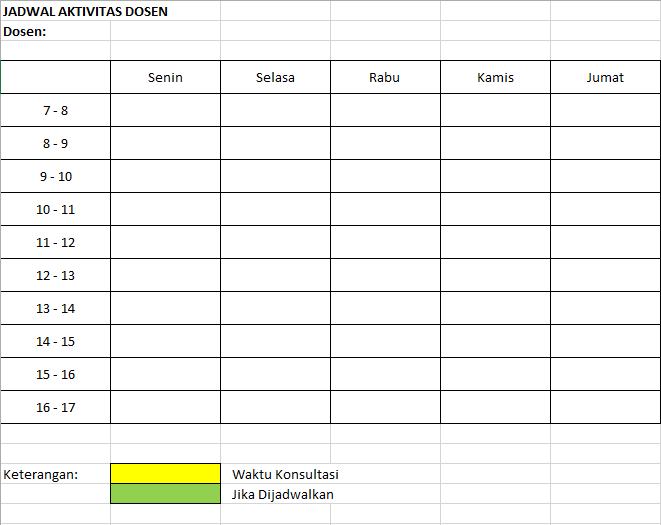
\includegraphics[scale=0.7]{template-jadwal-dosen.png}
\begin{figure} [h]
	\centering  
	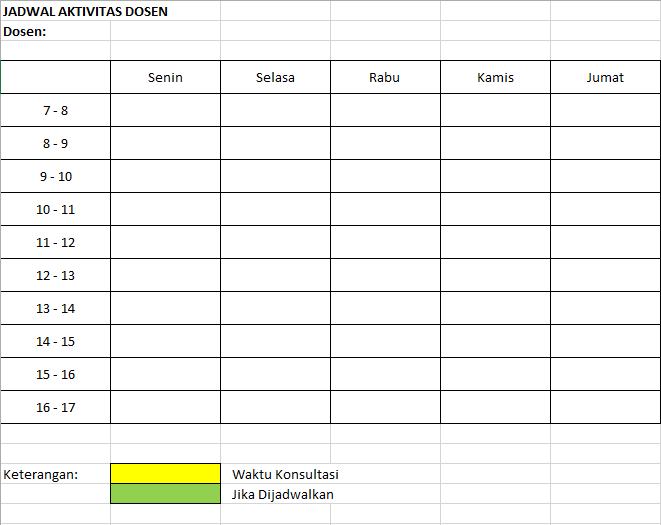
\includegraphics[scale=0.5]{template-jadwal-dosen.png}  
	\caption[Template jadwal dosen]{Template jadwal dosen} 
	\label{fig:template-jadwal-dosen} 
\end{figure} 
Jadwal tersebut akan ditempel pada dinding ruangan masing-masing dosen. Sedangkan bila menggunakan Blue Tape maka dosen tidak perlu lagi mencetak jadwalnya tersebut karena mahasiswa dapat melihat jadwal setiap dosen di dalam aplikasi ini. Maka dari itu aplikasi ini membuat pencatatan jadwal dosen menjadi \textit{papeless}.

%referensi pake unpublished

Pada Skripsi ini akan ditambahkan dua modul yaitu modul entri jadwal untuk dosen informatika dan modul lihat jadwal dosen untuk mahasiswa ke dalam aplikasi Blue Tape. Modul-modul tersebut berfungsi untuk melakukan hal-hal yang berhubungan dengan pembangkitan jadwal dosen. Modul dosen memiliki beberapa fungsi diantarnya: input jadwal mingguan dosen(jadwal dapat berupa jadwal konsultasi, jadwal konsultasi tentatif ataupun jadwal rutin), mencatat \textit{update} terakhir jadwal dosen dan mengekspor jadwal dosen ke XLS. Modul Umum sendiri memiliki fungsi untuk melihat jadwal seluruh dosen dan mengekspor jadwal dosen ke XLS.


\section{Rumusan Masalah}
\label{sec:rumusan}
Rumusan masalah yang akan dibahas dalam penelitian ini :
	\begin{enumerate}
		\item Bagaimana cara mencatat, \textit{update} dan melihat jadwal dosen di \textit{Blue Tape}?
		\item Bagaimana mengekspor jadwal dosen ke XLS sesuai template yang saat ini berlaku?
	\end{enumerate}


\section{Tujuan}
\label{sec:tujuan}
Tujuan yang ingin dicapai dalam penelitian ini : 
	\begin{enumerate}
		\item Membuat modul entri jadwal dosen dan modul lihat jadwal dosen yang berfungsi untuk menginput jadwal mingguan, \textit{update} dan melihat jadwal dosen
		\item Mengimplementasikan kode-kode yang diperlukan untuk memasukkan data yang ada di dalam PHP ke dalam \textit{file} XLS. 

	\end{enumerate}

\section{Batasan Masalah}
\label{sec:batasan}
Dalam penelitian ini ditetapkan batasan-batasan masalah sebagai berikut:
\begin{enumerate}
	\item Aplikasi ini tidak memeriksa hasil akhir bertipe file .xls, .xlsx atau tipe file lainnya.
	\item Aplikasi ini tidak mendukung fitur \textit{drag and drop}
	\item Aplikasi ini tidak mendukung fitur pemasukan jadwal dari sumber eksternal.
\end{enumerate}

\section{Metodologi}
\label{sec:metlit}
Metode penelitian yang akan digunakan dalam skripsi ini adalah:
\begin{enumerate}
   \item Studi literatur mengenai:
   		\begin{enumerate}
 		\item bahasa pemrograman PHP
 		\item \textit{framework} Codeigniter
 		\item modul \textit{Zurb Foundation} dan PHPExcel
		\end{enumerate}
   \item Analisis kebutuhan aplikasi dengan mengenali metode pencatatan jadwal dosen saat ini dan mengimplementasikannya ke dalam modul tersebut
    \item Membangun modul aplikasi yang sesuai dengan kebutuhan dosen dan mahasiswa dalam pembangkitan jadwal dosen agar aplikasi yang dibuat dapat membantu kedua pihak dalam mengakses informasi-informasi yang berkaitan dengan jadwal dosen . Pembuatan modul aplikasi ini dibagi menjadi empat tahap :
    	\begin{enumerate}
 		\item Analisis kebutuhan modul 
 		\item Perancangan modul
 		\item Implementasi 
 		\item Pengujian modul
		\end{enumerate}
\end{enumerate}
 

\section{Sistematika Pembahasan}
\label{sec:sispem}
Untuk penulisan skripsi ini akan dibagi dalam enam bagian sebagai berikut :

Bab 1 Pendahuluan berisi latar belakang, rumusan masalah, tujuan, batasan masalah,  metodologi penelitian dan sistematika penulisan.

Bab 2 Landasan Teori berisi dasar-dasar teori yang akan digunakan dalam pembuatan aplikasi pembangkit jadwal dosen. Dasar-dasar teori yang akan digunakan diantarnya adalah bahasa pemrograman PHP, framework Codeigniter, Google OAuth, CSRF, Zurb Foundation dan PHPExcel.

Bab 3 Analisis berisi analisis kebutuhan data, analisis sistem yang sudah ada sekarang dan analisis sistem usulan.

Bab 4 Perancangan berisi perancangan basis data, perancangan kelas-kelas program dan perancangan antarmuka program.

Bab 5 Implementasi dan Pengujian menjelaskan mengenai lingkungan yang digunakan dalam proses implementasi dan pengujian Aplikasi Pembangkit Jadwal Dosen. Bab ini juga mencatat hasil pengujian fungsional dan hasil pengujian eksperimental program.

Bab 6 Kesimpulan dan Saran berisi kesimpulan dari hasil pembuatan Aplikasi Pembangkit Jadwal Dosen ini dan kegunaannya, serta memberikan saran-saran untuk kelanjutan pengembangan aplikasi ini.
}{}
\ifdefstring{\vbabb}{1}{%versi 2 (8-10-2016)
\chapter{Landasan Teori}
\label{chap:teori}

\section{Codeigniter}
\label{sec:codeigniter} 
 
\paragraph{} Codeigniter adalah \textit{framework} pengembangan aplikasi untuk \textit{developer} yang membangun situs web menggunakan PHP. Tujuannya adalah untuk memungkinkan Anda mengembangkan proyek lebih cepat, daripada bila \textit{developer} menulis kode dari awal, dengan menyediakan banyak kumpulan \textit{library} untuk tugas-tugas yang sering dibutuhkan dan juga menyediakan tampilan sederhana serta struktur logika untuk mengakses \textit{library-library} tersebut. Codeigniter memungkinkan \textit{developer} untuk fokus secara kretif pada proyek \textit{developer} dengan cara meminimalkan jumlah kode yang dibutuhkan untuk setiap tugas yang diberikan.
\\
\\
Codeigniter dirancang untuk memenuhi kebutuhan :
\begin{itemize}
		\item \textit{Framework} dengan tapak keberadaan yang kecil
		\item performa yang baik
		\item kompabilitas akun \textit{hosting} yang luas yang dapat berjalan di berbagai versi dan konfigurasi PHP
		\item Framework yang hampir tidak membutuhkan konfigurasi
		\item \textit{Framework} yang tidak membutuhkan \textit{command line}
		\item Framework yang tidak mengikuti aturan pengkodean yang ketat
		\item membutuhkan solusi yang sederhana
		\item dokumentasi yang menyeluruh
	\end{itemize}
	
\subsection{Model-View-Controller}
Codeigniter didasari pola pengembangan \textit{Model-View-Controller} atau MVC. MVC memisahkan logika aplikasi dengan tampilannya.
\begin{itemize}
		\item \textbf{\textit{Model}} merepresentasikan struktur data. Pada umumnya kelas-kelas model menampung fungsi-fungsi untuk mengambil, memperbarui atau memasukan data ke dalam basis data.
		\item \textbf{\textit{View}} menampilkan informasi ke pengguna. 
		\item \textbf{\textit{Controller}} berfungsi sebagai perantara antara model dan view.
	\end{itemize}
Codeigniter menerapkan MVC secara longgar karena Model tidak diwajibkan ada. Developer dapat mengembangkan aplikasi dengan hanya menggunakan \textit{View} dan \textit{Controller} saja.

\subsection{Flow Chart Aplikasi}
Gambar dibawah mengilustrasikan aliran data dalam sistem :
\begin{figure} [ht]
	\centering  
	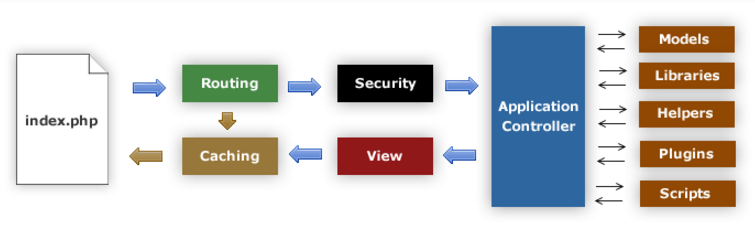
\includegraphics[scale=0.7]{appflowchart.png}  
	\caption[Flow Chart Aplikasi]{Flow Chart Aplikasi} 
	\label{fig:template-jadwal-dosen} 
\end{figure}
\begin{itemize}
		\item index.php berfungsi sebagai controller depan. Menginisialisasi sumber daya yang dibutuhkan untuk menjalankan Codeigniter
		\item Router memeriksa permintaan HTTP untuk menentukan apa yang akan dilakukan pada permintaan tersebut.
		\item Jika ada cache file, maka akan dikirim langsung ke browser. Melewati cara eksekusi sistem yang normal.
		\item Security. Sebelum controller aplikasi dimuat, permintaan HTTP dan data-data pengguna yang telah diserahkan disaring untuk kemanan.
		\item Controller memuat model, pustaka inti (\textit{core libraries}), pembantu dan sumber daya lain yang dibutuhkan untuk memproses permintaan khusus.
		\item Kemudian tampilan akhir dibuat dan dikirim ke web browser untuk dilihat. Jika caching diaktifkan, maka tampilan dimasukan ke dalam cache terlebih dahulu sehingga pada permintaan selanjutnya tampilan tersebut dapat diakses lebih cepat.
	\end{itemize}
	

\section{Zurb Foundation}
\label{zurbfoundation}

\paragraph{}  }{}
\ifdefstring{\vbabc}{1}{%versi 2 (8-10-2016)-pppppppppppppp;
\chapter{Analisis}
\label{chap:analisis}
\setcounter{secnumdepth}{3}

\paragraph{} Pengumpulan data dalam skripsi ini dilakukan dengan cara studi pustaka untuk mempelajari cara pengembangan perangkat lunak menggunakan \textit{Framework} BlueTape yang berbasis CodeIgniter. Selain itu juga dipelajari \textit{library-library} pembantunya diantara lain : PHPExcel , Google OAuth dan ZurbFoundation. Tujuan studi pustaka ini untuk memahami secara rinci cara-cara untuk menambahkan layanan berbentuk modul ke dalam BlueTape dan membangun layanan tersebut menggunakan \textit{library-library} yang disebutkan sebelum ini.

\section{Analisis Sistem Kini}
\paragraph{} Aplikasi \textit{Blue Tape} adalah perangkat lunak \textit{open source} sederhana yang memiliki tujuan utama untuk mengubah berbagai pekerjaan \textit{paper-based} di FTIS UNPAR menjadi \textit{paperless}. Selain itu perangkat lunak ini memiliki beberapa kegunaan lainnya seperti mengautentikasi mahasiswa dan staf UNPAR via OAuth 2.0 ke Google (layanan OAuth ke Google ini juga dapat digunakan untuk menentukan hak akses yang bisa dilihat dari email pengguna) dan \textit{Pilot Project} untuk permohonan transkrip ke Tata Usaha . Aplikasi ini merupakan aplikasi berbasis web dengan memanfaatkan \textit{Codeigniter} dan \textit{Zurb Foundation}. 
\newline
\begin{figure} [H]
	\centering  
	\frame{
\includegraphics[scale=0.4]{halamanUtama.png}}
	\caption[Halaman Utama BlueTape Untuk Login dan Membuka Petunjuk Penggunaan]{Halaman Utama BlueTape Untuk Login dan Membuka Petunjuk Penggunaan} 
	\label{fig:flow-chart-CodeIgniter} 
\end{figure}
Perangkat lunak \textit{Blue Tape} ini didesain sebagai \textit{framework} yang terdiri dari beberapa layanan yang dipisahkan ke dalam modul-modul. Pemisahan layanan ke dalam modul-modul dibuat dengan tujuan agar pemeliharan perangkat lunak lebih mudah dan juga mempermudah cara untuk menambahkan layanan baru ke dalam BlueTape. Sudah ada layanan yang aktif di BlueTape saat ini yaitu \textit{Transcript Request / Manage} yang memiliki fungsi untuk melakukan permohonan serta pencetakan transkrip mahasiswa.

\subsection{\textit{Transcript Request / Manage}}
\paragraph{} Modul \textit{Transcript Request/Manage} merupakan salah satu dari dua modul yang sudah aktif di BlueTape ketika skripsi ini ditulis. Modul ini memiliki fungsi utama sebagai alat bagi mahasiswa untuk memohon pencetakan transkrip ke Tata Usaha dengan tampilan seperti di bawah ini :
\begin{figure} [H]
	\centering  
	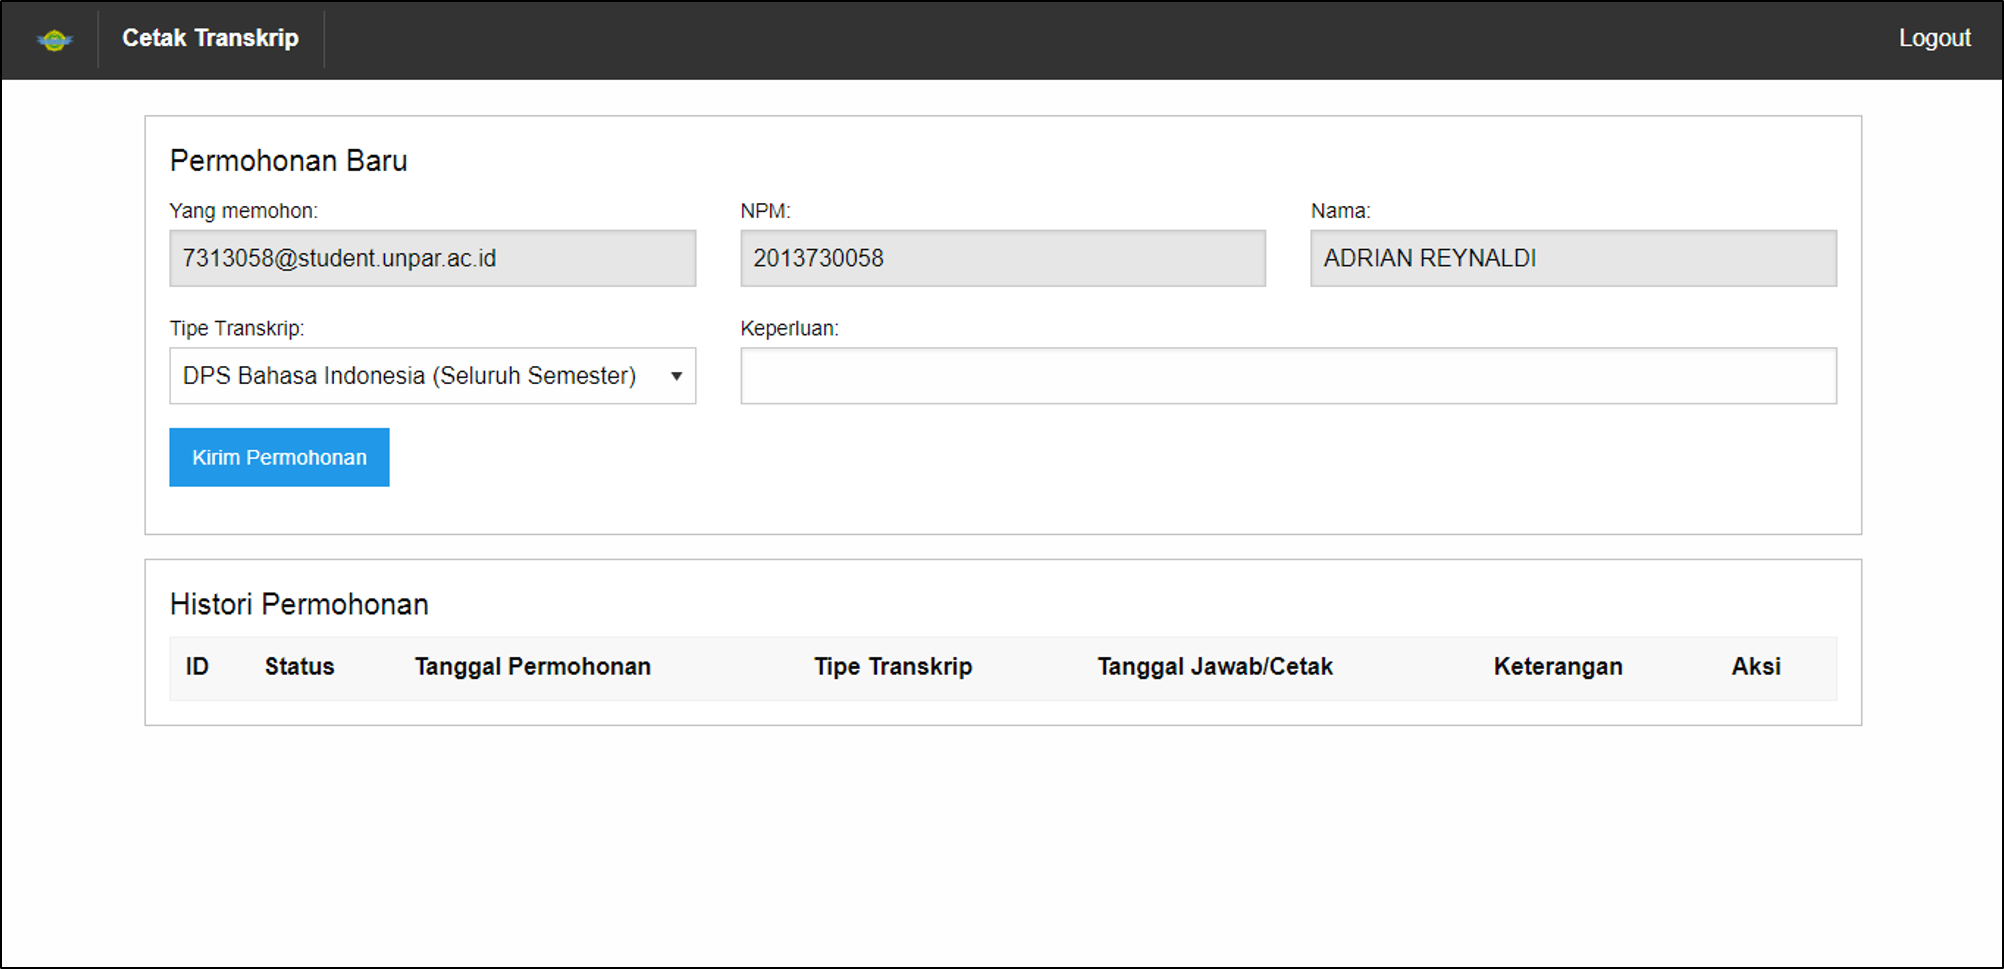
\includegraphics[scale=0.48]{cetakTranskrip.png}
	\caption[Tampilan Cetak Transkrip]{Tampilan Cetak Transkrip} 
	\label{fig:flow-chart-CodeIgniter} 
\end{figure}
\begin{figure} [H]
	\centering  
	\frame{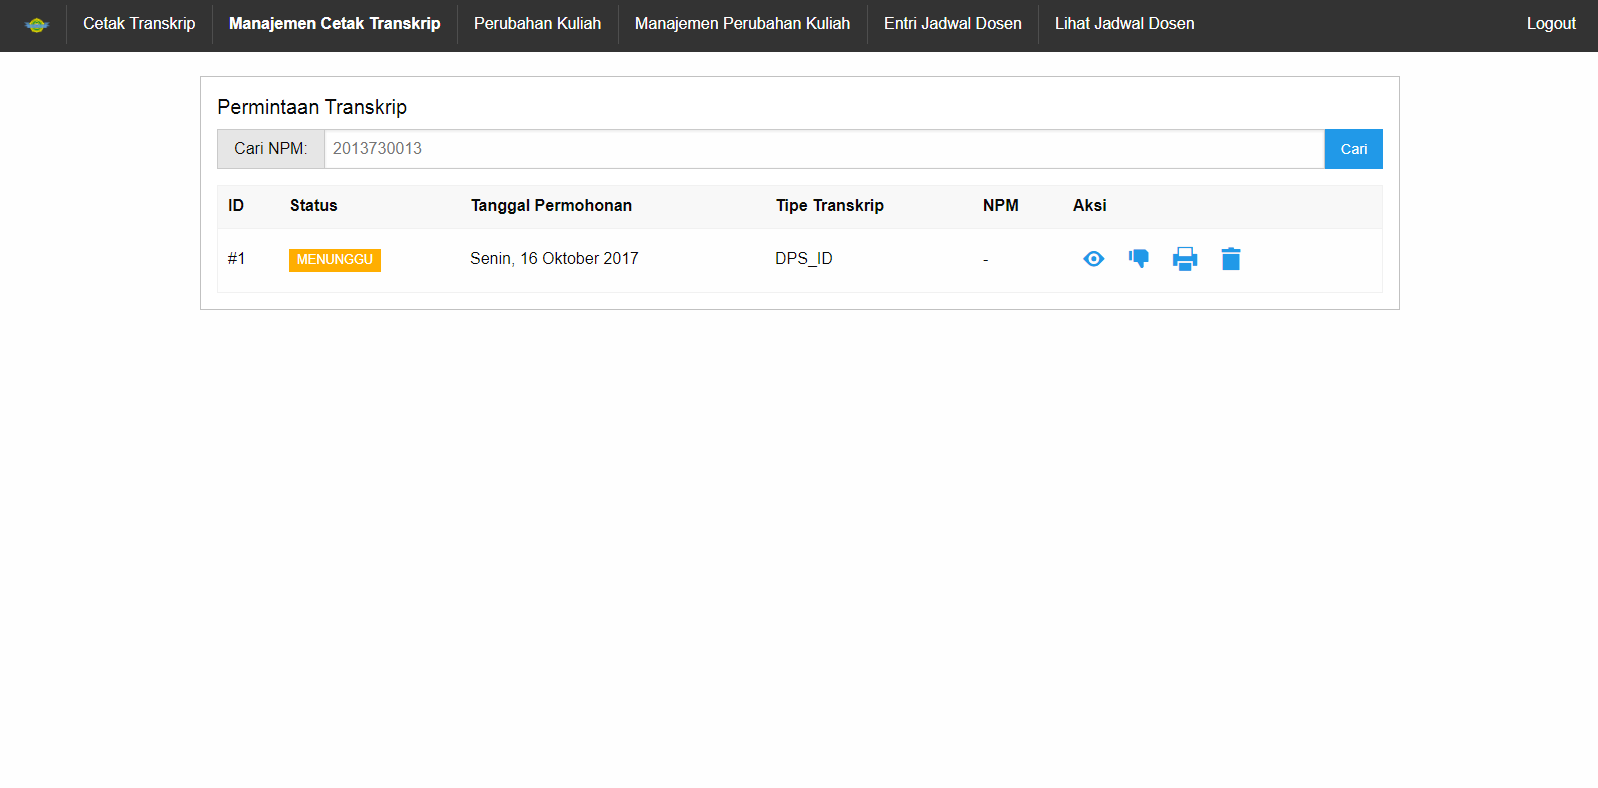
\includegraphics[scale=0.4]{manageTranskrip.png}}
	\caption[Tampilan Manajemen Transkrip]{Tampilan Manajemen Transkrip} 
	\label{fig:flow-chart-CodeIgniter} 
\end{figure}
Untuk memohon pencetakan transkrip pada halaman tersebut mahasiswa diperlukan untuk melakukan :
\begin{enumerate}
  \item Memilih salah satu dari 3 tipe transkrip yang ada. Ada 3 tipe transkrip: Daftar Perkembangan Studi (DPS) Bahasa Inggris, DPS Bahasa Indonesia dan Lembar Hasil Studi Semester Akhir.
  \item Lalu mahasiswa mengisi keterangan keperluan pencetakan transkrip di \textit{field} keperluan.
  \item Setelah kedua hal tersebut dipilih dan diisi , tekan tombol "Kirim Permohonan" untuk memohon pencetakan transkrip ke Tata Usaha.
\end{enumerate}
Tata usaha memiliki beberapa opsi untuk merespon permintaan yang sudah dikirim mahasiswa tadi :
\begin{enumerate}
	\item Melihat detail permintaan transkrip
	\item Menolak permintaan transkrip
	\item Mencetak detail permintaan transkrip
	\item Menghapus permintaan transkrip
\end{enumerate}

\subsection{Perubahan Kuliah}
\paragraph{} Perubahan kuliah adalah modul kedua yang sudah aktif di BlueTape. Modul ini berfungsi sebagai alat bagi mahasiswa untuk mengirimkan permintaan perubahan kuliah dari mahasiswa ke karyawan tata usaha. Selain itu karyawan tata usaha juga dapat menggunakan modul ini untuk mengatur permintaan-permintaan yang sudah dikirim dari mahasiswa tadi. 
\begin{figure} [H]
	\centering  
	\frame{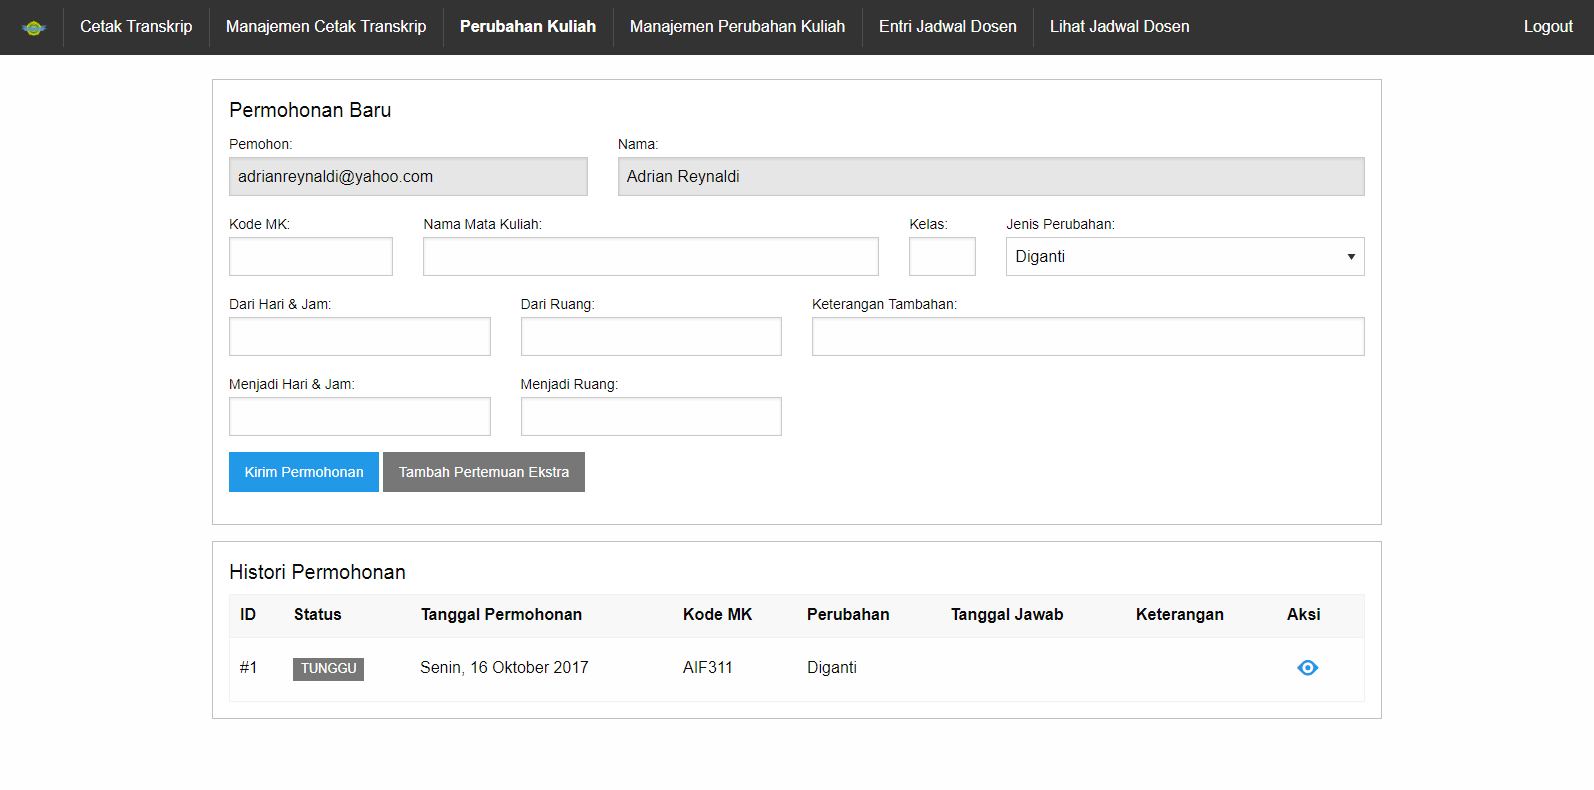
\includegraphics[scale=0.4]{perubahanKuliah.png}}
	\caption[Tampilan Menu Perubahan Kuliah]{Tampilan Menu Perubahan Kuliah} 
	\label{fig:flow-chart-CodeIgniter} 
\end{figure}
\begin{figure} [H]
	\centering  
	\frame{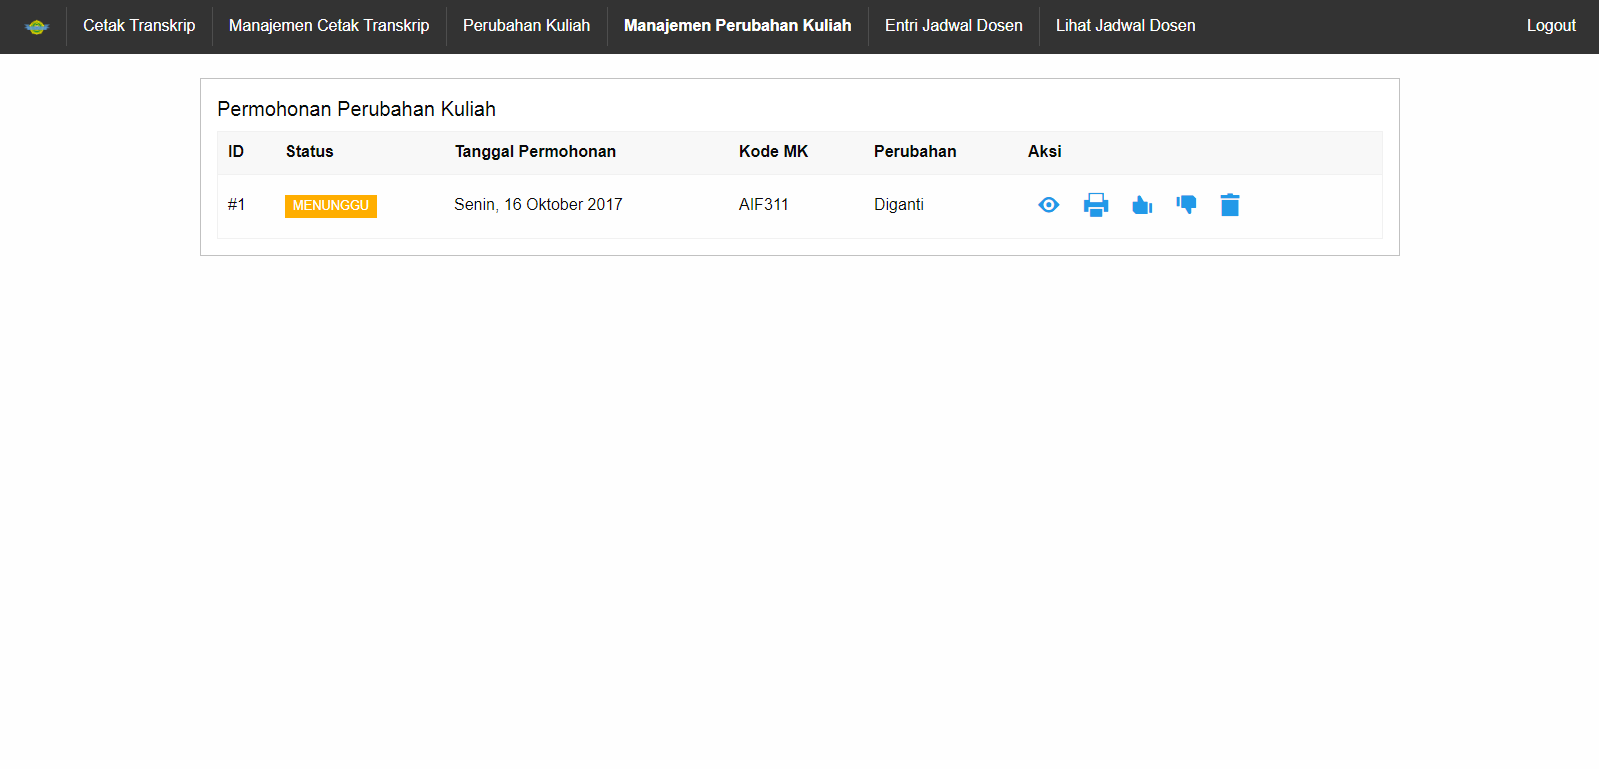
\includegraphics[scale=0.4]{managePerubahanKuliah.png}}
	\caption[Tampilan Menu Manajemen Perubahan Kuliah]{Tampilan Menu Manajemen Perubahan Kuliah} 
	\label{fig:flow-chart-CodeIgniter} 
\end{figure}
Untuk membuat permintaan perubahan kuliah, mahasiswa perlu mengisi setiap \textit{field} yang ada di menu. Setelah semua \textit{field} diisi, mahasiswa bisa memilih untuk mengirim permohonan atau tambah pertemuan.
\begin{itemize}
	\item Tombol "Kirim Permohonan" akan memeriksa apakah data yang sudah dimasukan sudah benar, bila sudah maka data permohonan akan dikrim ke server dan apabila ada yang masih salah maka sistem akan menandai bagian yang salah.
	
	\item Tombol "Tambah Pertemuan Ekstra" akan memunculkan 2 \textit{field} baru yaitu \textit{field} "Menjadi Hari dan jam" dan \textit{field} "Menjadi Ruang". Bila mahasiswa ingin mengirimkan permintaan penambahan pertemuan, tetap harus menekan tombol "Kirim Permohonan" setelah kedua \textit{field} yang baru tersebut juga diisi.
\end{itemize}
Di sisi tata usaha , modul ini memiliki fungsi untuk :
\begin{itemize}
	\item Menolak permintaan perubahan kuliah
	\item Menyetujui permintaan perubahan kuliah
	\item Mencetak detail perubahan kuliah
	\item Melihat detail perubahan kuliah
	\item Menghapus permintaan perubahan kuliah
\end{itemize}
  
\subsection{Pengguna Aplikasi}
Pada bagian ini akan dijelaskan pengelompokan tipe-tipe pengguna aplikasi BlueTape.

\subsubsection{Mahasiswa FTIS}
Mahasiswa FTIS adalah semua mahasiswa Fakultas Teknik Informasi dan Sains. Saat ini golongan Mahasiwa FTIS baru memiliki satu akses yaitu untuk memnita transkrip.


\subsubsection{Tata Usaha UNPAR}
Tata Usaha UNPAR adalah golongan pengguna yang bekerja sebagai staff tata usaha di Universitas Katolik Parahyangan. Di BlueTape, Tata Usaha UNPAR memilki akses fitur-fitur sebagai berikut :
\begin{itemize}
	\item Mengatur permintaan transkrip dari mahasiswa
	\item Mengatur permintaan perubahan kuliah 
\end{itemize}

\subsubsection{Staf UNPAR}
Staf UNPAR adalah para pekerja dan karyawan di Universitas Katolik Parahyangan. Untuk saat ini golongan staf UNPAR hanya memiliki akses fitur untuk meminta perubahan kuliah.

\subsubsection{Mahasiswa Informatika}
Mahasiswa Informatika adalah pengguna yang memiliki kepentingan untuk mencetak transkrip nilai. Di Bluetape saat ini, Mahasiswa Informatika baru memiliki satu fitur yaitu untuk meminta transkrip nilai.


\subsection{Diagram Use Case Sistem Kini}
\begin{figure} [H]
	\centering  
	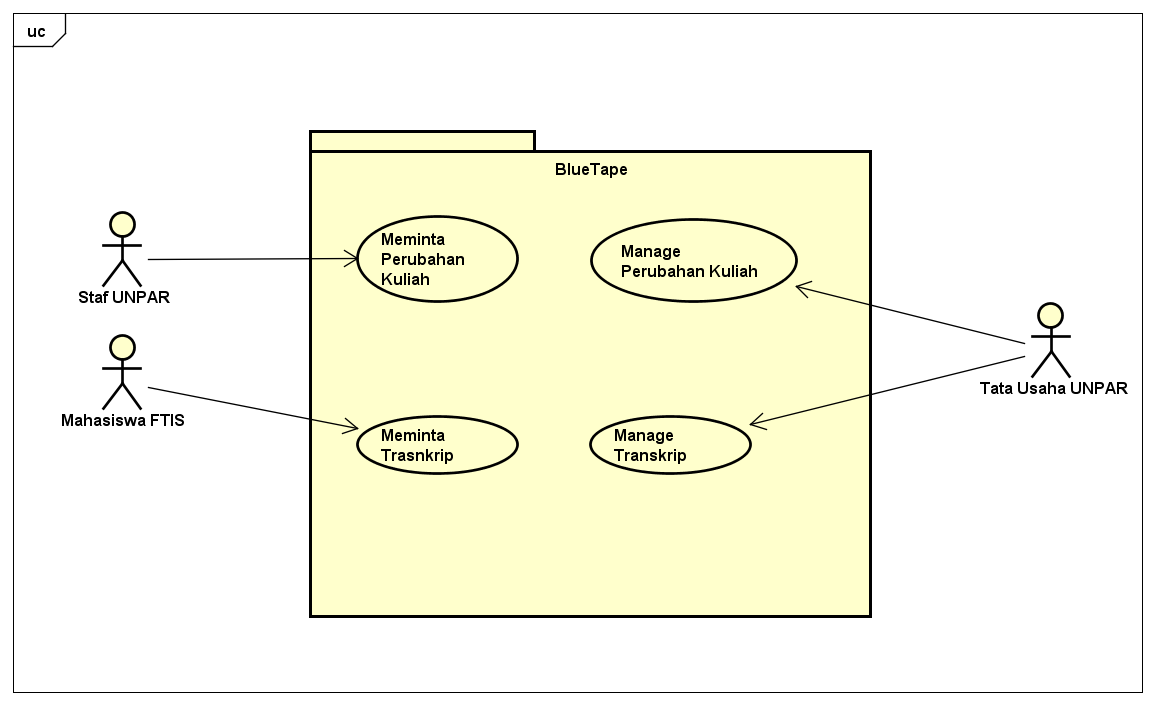
\includegraphics[scale=0.48]{useCaseDiagramAwal.png}
	\caption[Diagram Use Case Sistem Kini]{Diagram Use Case Sistem Kini} 
	\label{fig:flow-chart-CodeIgniter} 
\end{figure}
Berikut ini adalah penjelasan skenario dari diagram \textit{use case} dari Gambar 3.6 atas:

\begin{enumerate}
	\item Skenario Meminta Perubahan Kuliah
	\begin{itemize}
		\item Aktor : Staf UNPAR, Tata Usaha UNPAR
		\item Skenario Normal
			\begin{enumerate}[1.]
				\item Staf UNPAR mengisi data-data yang diperlukan untuk melakukan perubahan kuliah
				\item Sistem mengirim data-data tersebut ke server 
				\item Tata Usaha menerima data yang dikirim oleh Staf UNPAR untuk diproses
			\end{enumerate}
		\item Skenario \textit{Exception}
			\begin{enumerate}[1.]
			 	\item Staf UNPAR memasukan data secara tidak lengkap
			 	\item Sistem menampilkan pesan eror karena data tidak lengkap
			\end{enumerate}
	\end{itemize}


	\item Skenario Melihat Detail Perubahan Kuliah
	\begin{itemize}
		\item Aktor : Tata Usaha UNPAR
		\item Skenario Normal
			\begin{enumerate}[1.]
				\item Aktor memilih data perubahan kuliah 
				\item Aktor memilih menu lihat detail
				\item Sistem menampilkan semua data-data permintaan mahasiswa dengan npm terkait 
			\end{enumerate}
	\end{itemize}
	
	\item Skenario Menolak Perubahan Kuliah 
	\begin{itemize}
		\item Aktor : Staf UNPAR, Tata Usaha UNPAR
		\item Skenario Normal
			\begin{enumerate}[1.]
				\item Tata Usaha UNPAR memilih data perubahan kuliah 
				\item Tata Usaha UNPAR memilih menu tolak perubahan kuliah
				\item Tata Usaha UNPAR mengisi data alasan penolakan
				\item Sistem mengirim pesan berisi alasan penolakan ke staf UNPAR
				\item Sistem menghapus permintaan perubahan kuliah dari \textit{database}
			\end{enumerate}
	\end{itemize}
	
	\item Skenario Menyetujui Perubahan Kuliah 
	\begin{itemize}
		\item Aktor : Staf UNPAR, Tata Usaha UNPAR
		\item Skenario Normal
			\begin{enumerate}[1.]
				\item Tata Usaha UNPAR memilih data perubahan kuliah 
				\item Tata Usaha UNPAR memilih menu tolak perubahan kuliah
				\item Tata Usaha UNPAR mengisi keterangan penyetujuan
				\item Sistem mengirim pesan berisi keterangan penyetujuan ke staf UNPAR
				\item Sistem menghapus permintaan perubahan kuliah dari \textit{database}
			\end{enumerate}
	\end{itemize}
	
	\item Skenario Menghapus Perubahan Kuliah 
	\begin{itemize}
		\item Aktor : Tata Usaha UNPAR
		\item Skenario Normal
			\begin{enumerate}[1.]
				\item Tata Usaha UNPAR memilih data perubahan kuliah 
				\item Tata Usaha UNPAR memilih menu hapus
				\item Sistem menghapus permintaan perubahan kuliah dari \textit{database}
			\end{enumerate}
	\end{itemize}

\item Skenario Cetak Detail Perubahan Kuliah 
	\begin{itemize}
		\item Aktor : Tata Usaha UNPAR
		\item Skenario Normal
			\begin{enumerate}[1.]
				\item Tata Usaha UNPAR memilih data perubahan kuliah 
				\item Tata Usaha UNPAR memilih menu cetak
				\item Sistem mencetak detail permintaan perubahan kuliah
			\end{enumerate}
	\end{itemize}
%=========================================================

	\item Skenario Meminta Transkrip
	\begin{itemize}
		\item Aktor : Mahasiswa FTIS
		\item Skenario Normal
			\begin{enumerate}[1.]
				\item Mahasiswa FTIS mengisi data keterangan dan tipe transkrip 
				\item Sistem menyimpan data-data tersebut ke server 
			\end{enumerate}
	\end{itemize}
	
	\item Skenario Lihat Detail Permintaan Transkrip
	\begin{itemize}
		\item Aktor : Tata Usaha UNPAR
		\item Skenario Normal
			\begin{enumerate}[1.]
				\item Tata Usaha UNPAR memilih data permintaan
				\item Tata Usaha UNPAR memilih menu lihat detail
				\item Sistem menampilkan detail data permintaan
			\end{enumerate}
	\end{itemize}
	
	\item Tolak Permintaan Transkrip
	\begin{itemize}
		\item Aktor : Tata Usaha UNPAR
		\item Skenario Normal
			\begin{enumerate}[1.]
				\item Tata Usaha UNPAR memilih data permintaan
				\item Tata Usaha UNPAR memilih menu tolak permintaan
				\item Sistem menampilkan menu keterangan penolakan
				\item Tata Usaha UNPAR mengisi data keterangan penolakan
				\item Sistem mengirim pesan berisi keterangan penolakan ke Mahasiswa FTIS.
			\end{enumerate}
	\end{itemize}
	
	\item Hapus Permintaan Transkrip
	\begin{itemize}
		\item Aktor : Tata Usaha UNPAR
		\item Skenario Normal
			\begin{enumerate}[1.]
				\item Tata Usaha UNPAR memilih data permintaan
				\item Tata Usaha UNPAR memilih menu hapus
				\item Sistem menampilkan pesan konfirmasi
				\item Tata Usaha UNPAR mengkonfirmasi penghapusan
				\item Sistem menghapus data permintaan dari \textit{database}
			\end{enumerate}
	\end{itemize}

%==========================================================
	
\end{enumerate}

\section{Analisis Sistem Usulan: Aplikasi Pembangkit Jadwal Dosen}
Aplikasi Pembangkit Jadwal Dosen adalah aplikasi tambahan untuk BlueTape yang memiliki dua modul yaitu:
\begin{enumerate}
	\item Modul Entri Jadwal Dosen yang bisa melakukan:
		\begin{itemize}
			\item Input jadwal mingguan
			\item Mencatat update terakhir
			\item Ekspor jadwal ke XLS
		\end{itemize}
	\item Modul Lihat Jadwal Dosen yang bisa melakukan:
		\begin{itemize}
			\item Melihat jadwal-jadwal semua dosen
			\item Ekspor jadwal ke XLS
		\end{itemize}
\end{enumerate}
Untuk mengimplementasikan fitur-fitur tersebut maka digunakan teknologi:
\begin{itemize}
	\item PHP \& CodeIgniter
	\item Zurb Foundation
	\item Framework BlueTape
	\item Google OAuth
	\item PHPExcel
\end{itemize}

\subsection{Diagram Use Case Sistem Usulan}
\begin{figure} [H]
	\centering  
	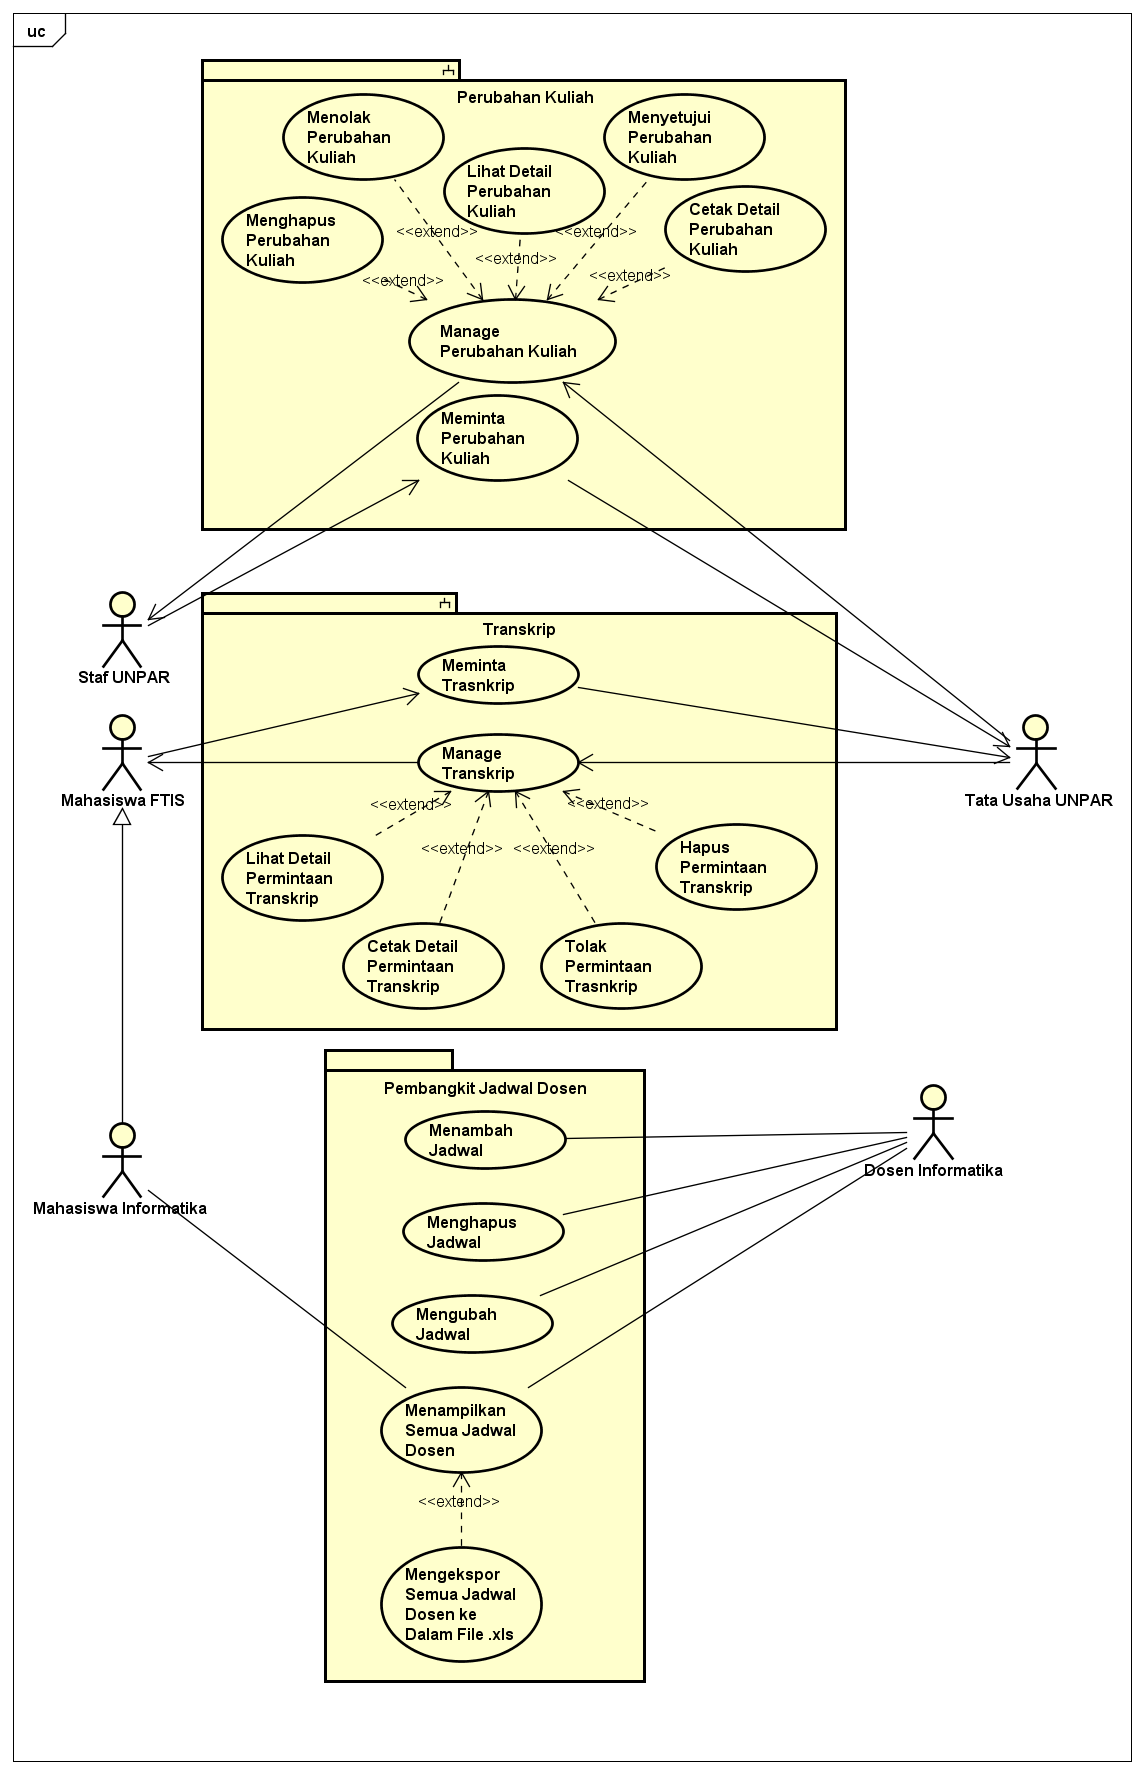
\includegraphics[scale=0.48]{useCaseDiagramSemua.png}
	\caption[Diagram Use Case Sistem Usulan]{Diagram Use Case Sistem Usulan} 
	\label{fig:flow-chart-CodeIgniter} 
\end{figure}

Tidak ada perubahan pada diagram \textit{usecase} dan skenario dari sistem kini (bisa dilihat pada Gambar 3.6) hanya ditambahkan bagian untuk Aplikasi Pembangkit Jadwal Dosen. Berikut ini adalah penjelasan skenario yang ditambahkan dari diagram \textit{usecase} pada Gambar 3.7:
\begin{enumerate}
	\item Skenario Menambah Jadwal
	\begin{itemize}
		\item Aktor : Dosen Informatika
		\item Skenario Normal
			\begin{enumerate}[1.]
				\item Dosen Informatika mengisi data jadwal
				\item Sistem menyimpan data jadwal tersebut ke dalam \textit{database}
			\end{enumerate}
	\end{itemize}

	\item Skenario Mengubah Jadwal
	\begin{itemize}
		\item Aktor : Dosen Informatika
		\item Skenario Normal
			\begin{enumerate}[1.]
				\item Dosen Informatika memilih jadwal yang akan diubah
				\item Sistem menampilkan menu pengubahan berisi data jadwal yang dipilih tadi
				\item Dosen Informatika mengubah data-data yang ingin diubah
				\item Sistem menyimpan hasil perubahan ke dalam database
			\end{enumerate}
	\end{itemize}


	\item Skenario Menghapus Jadwal
	\begin{itemize}
		\item Aktor : Dosen Informatika
		\item Skenario Normal
			\begin{enumerate}[1.]
				\item Dosen Informatika memilih jadwal yang akan dihapus
				\item Sistem menampilkan menu pengubahan berisi data jadwal yang dipilih
				\item Dosen Informatika menekan tombol hapus
				\item Sistem menghapus data jadwal tersebut yang ada di database
			\end{enumerate}
	\end{itemize}

	\item Skenario Menampilkan Semua Jadwal Dosen
	\begin{itemize}
		\item Aktor : Mahasiswa Informatika , Dosen Informatika
		\item Skenario Normal
			\begin{enumerate}[1.]
				\item Aktor memilih menu lihat jadwal dosen
				\item Sistem memuat semua data jadwal-jadwal dari \textit{database}
				\item Sistem mengelompokan setiap jadwal berdasarkan pemiliknya
				\item Sistem membuat tab-tab yang merepresentasikan setiap dosen yang sudah menyimpan jadwal ke dalam database
				\item Sistem memasukan jadwal-jadwal ke dalam tab-tab sesuai nama pemiliknya.
			\end{enumerate}
	\end{itemize}
	

	\item Skenario Mengekspor Semua Jadwal Dosen ke Dalam File .xls
	\begin{itemize}
		\item Aktor : Mahasiswa Informatika , Dosen Informatika
		\item Skenario Normal
			\begin{enumerate}[1.]
				\item Aktor memilih menu lihat jadwal dosen
				\item Sistem memuat semua data jadwal-jadwal dari \textit{database}
				\item Sistem mengelompokan setiap jadwal berdasarkan pemiliknya
				\item Sistem membuat tab-tab yang merepresentasikan setiap dosen yang sudah menyimpan jadwal ke dalam database
				\item Sistem memasukan jadwal-jadwal ke dalam tab-tab sesuai nama pemiliknya.
				\item Aktor menekan tombol ekspor
				\item Sistem mengkonversi semua data jadwal dari bentuk php ke dalam bentuk \textit{spreadsheet} .xls
				\item Sistem menampilkan menu pemilihan lokasi penyimpanan \textit{file} .xls
				\item Aktor menekan tombol simpan
				\item Sistem menyimpan file .xls tersebut di lokasi yang sudah dipilih oleh aktor.
			\end{enumerate}
		\item Skenario Exception
			\begin{enumerate}[1.]
				\item Aktor memilih menu lihat jadwal dosen
				\item Sistem memuat semua data jadwal-jadwal dari \textit{database}
				\item Sistem tidak menerima data apapun dari \textit{database}
				\item Sistem men-\textit{disable} tombol ekspor
			\end{enumerate}
	\end{itemize}
\end{enumerate}

\subsection{Pengguna Aplikasi}
Pada bagian ini akan dijelaskan pengelompokan tipe-tipe pengguna aplikasi BlueTape dengan sistem usulan. Perubahan terjadi pada kelompok "Mahasiswa Informatika" yang mendapat fitur tambahan. Selain itu , ada penambahan kelompok pengguna yaitu "Dosen Informatika". Perubahan-perubahan akan dijelaskan pada bagian masing-masing.

\subsubsection{Mahasiswa FTIS}
Mahasiswa FTIS adalah semua mahasiswa Fakultas Teknik Informasi dan Sains. Saat ini golongan Mahasiwa FTIS baru memiliki satu akses yaitu untuk memnita transkrip.


\subsubsection{Tata Usaha UNPAR}
Tata Usaha UNPAR adalah golongan pengguna yang bekerja sebagai staff tata usaha di Universitas Katolik Parahyangan. Di BlueTape, Tata Usaha UNPAR memilki akses fitur-fitur sebagai berikut :
\begin{itemize}
	\item Mengatur permintaan transkrip dari mahasiswa
	\item Mengatur permintaan perubahan kuliah 
\end{itemize}

\subsubsection{Staf UNPAR}
Staf UNPAR adalah para pekerja dan karyawan di Universitas Katolik Parahyangan. Untuk saat ini golongan staf UNPAR hanya memiliki akses fitur untuk meminta perubahan kuliah.

\subsubsection{Mahasiswa Informatika}
Mahasiswa Informatika adalah pengguna yang memiliki kepentingan untuk melihat jadwal-jadwal semua dosen Informatika. Dengan mengetahui jadwal dosen, maka mahasiswa dapat mengatur jadwal bimbingan atau konsultasi lainnya dengan dosen terkait secara lebih teratur. 
\begin{itemize}
	\item Melihat semua jadwal dosen Informatika
	\item Mengekspor semua jadwal dosen Informatika ke dalam tipe file .xls
	\item Meminta transkrip nilai
\end{itemize}

\subsubsection{Dosen Informatika}
Dosen merupakan pengguna yang dapat memasukan jadwal-jadwalnya ke dalam BlueTape agar dapat dilihat mahasiswa. Dosen memilki akses pada fitur :
\begin{itemize}
	\item Memasukan jadwal ke dalam BlueTape
	\item Mengubah jadwal yang sudah dimasukan  
	\item Menghapus jadwal yang sudah dimasukan
	\item Melihat semua jadwal dosen , termasuk jadwal miliknya sendiri
	\item Mengeskpor semua jadwal dosen ke dalam tipe file .xls
\end{itemize}}{}
\ifdefstring{\vbabd}{1}{%versi 2 (8-10-2016)-pppppppppppppp;
\chapter{Perancangan dan Implementasi}
\label{chap:perancanganDanImplementasi}
\setcounter{secnumdepth}{3}

\paragraph{}
\section{Perancangan Basis Data}
\subsection{Model Relasional}
Dari analisis yang telah dilakukan, maka dibuatlah model relasional seperti pada gambar 4.1

\begin{figure} [H]
	\centering  
	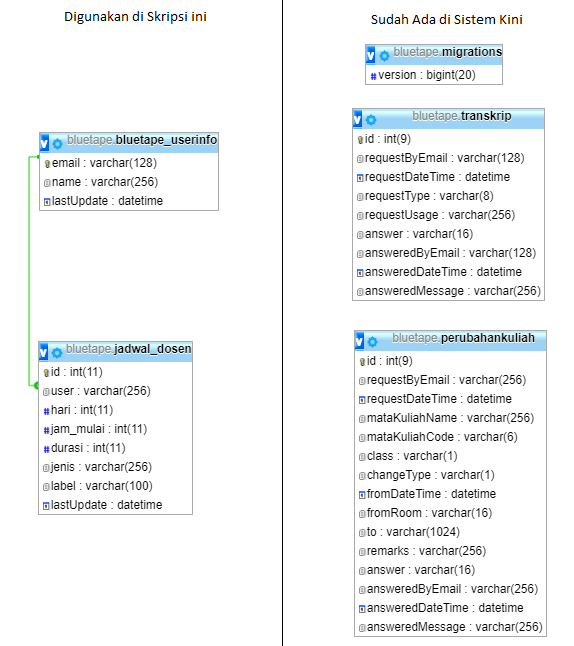
\includegraphics[scale=0.9]{ERDiagram.png}  
	\caption[Model Realsional]{Model Realsional} 
	\label{fig:skematik-phpexcel} 
\end{figure}

\subsection{Perancangan Tabel}
\begin{center}
	\begin{table}[H]
	\begin{tabular}{|c|c|c|c|c|c|c|}
 			\hline
		\textbf{Atribut} & \textbf{Tipe Data} & \textbf{Ukuran} & \textbf{Primary Key} & \textbf{Foreign Key} & \textbf{Null} & \textbf{Keterangan} \\
			\hline
		 id & int & 11 & ya & tidak & tidak & id jadwal\\
			 \hline
			 user & varchar & 256 & tidak & ya & tidak & pemilik jadwal\\
			 \hline
			 hari & int & 11 & tidak & tidak & tidak & hari berlangsungnya jadwal\\
			 \hline
			 jam\_mulai & int & 11 & tidak & tidak & tidak & jam berlangsungnya jadwal\\
			 \hline
			 durasi & int & 11 & tidak & tidak & tidak & lama jadwal berlangsung\\
			 \hline
			 jenis & varchar & 255 & tidak & tidak & tidak & jenis kegiatan jadwal\\
			 \hline
			 label & varchar & 100 & ya & tidak & tidak & nama kegiatan\\
			 \hline
	\end{tabular}
	\caption{Perancangan Tabel Jadwal}
	\end{table}
\end{center}

\subsection{Perancangan Rinci}
\subsubsection{Controller EntriJadwalDosen}
\paragraph{} Berikut adalah perancangan kelas Controller EntriJadwalDosen \\
\begin{tabular}{|c|p{11cm}|}
\hline
Nama Method 	& 	insert 	\\
\hline
Parameter Output & insert\_success, insert\_failed \\
\hline
Tabel yang berhubungan & jadwal\_dosen \\
\hline
Deskripsi	& Proses untuk memasukan jadwal \\
\hline
Algoritma	& \begin{itemize}
				\item proses menerima input-input data dari user
				\item proses mengecek apakah data-data yang dimasukan sudah valid
				\item proses mengecek apakah jadwal yang bertabrakan dengan jadwal lain atau tidak
				\item bila jadwal bertabrakan dengan jadwal lain maka proses menampilkan pesan "Jadwal gagal dimasukan. Sudah ada jadwal lain pada waktu ini"
				\item bila tidak ada masalah , proses akan memasukan data ke dalam database
				\end{itemize} \\
\hline
\end{tabular}
\\

\begin{tabular}{|c|p{11cm}|}
\hline
Nama Method 	& 	edit 	\\
\hline
Parameter Output & edit\_success, edit\_failed \\
\hline
Tabel yang berhubungan & jadwal\_dosen \\
\hline
Deskripsi	& Proses untuk mengubah jadwal yang sudah dimasukan sebelumnya \\
\hline
Algoritma	& \begin{itemize}
				\item proses menerima input-input data dari user
				\item proses mengecek apakah data-data yang dimasukan sudah valid
				\item proses mengecek apakah waktu baru dari jadwal yang diubah bertabrakan dengan jadwal lain atau tidak
				\item bila jadwal bertabrakan dengan jadwal lain maka proses menampilkan pesan "Pengubahan gagal. Sudah ada jadwal lain pada waktu ini"
				\item bila tidak ada masalah, maka jadwal akan memperbarui data yang ada di database.
				\end{itemize} \\
\hline
\end{tabular}
\\

\begin{tabular}{|c|p{11cm}|}
\hline
Nama Method 	& 	delete 	\\
\hline
Parameter Output & deleted \\
\hline
Tabel yang berhubungan & jadwal\_dosen \\
\hline
Deskripsi	& Proses untuk menghapus jadwal \\
\hline
Algoritma	& \begin{itemize}
				\item proses menerima pilihan jadwal yang akan dihapus oleh user.
				\item proses mengeluarkan form konfirmasi untuk memastikan user untuk menghapus jadwal yang bersangkutan
				\item bila user memilih "ya", maka data jadwal yang bersangkutan akan dihapus dari database.
				\item bila pilihan user "tidak" maka proses akan menampilkan halaman sebelum user menekan tombol \textit{delete}.
				\end{itemize} \\
\hline
\end{tabular}


\subsubsection{Controller LihatJadwalDosen}
\paragraph{} Berikut adalah perincian rancangan kelas Controller LihatJadwalDosen \\
\begin{tabular}{|c|p{11cm}|}
\hline
Nama Method 	& 	index 	\\
\hline
Parameter Output & - \\
\hline
Tabel yang berhubungan & jadwal\_dosen \\
\hline
Deskripsi	& Proses untuk memperlihatkan jadwal ke user \\
\hline
Algoritma	& \begin{itemize}
				\item proses memuat semua data jadwal dari database.
				\item proses mengelompokan jadwal-jadwal dari database tersebut berdasarkan pemiliknya.
				\item proses membuat tab-tab setiap tab diberi nama dosen yang sudah memasukan jadwal ke dalam sistem
				\item proses memasukan setiap jadwal yang sudah dipisahkan berdasarkan pemilik ke dalam tab-tab sesuai dengan nama pemilik yang bersangkutan.
				\item secara default akan ditampilkan jadwal dosen yang pertama kali dimuat oleh proses.
				\item bila user menekan tab, proses akan menampilkan semua jadwal dosen terkait
				\end{itemize} \\
\hline
\end{tabular}
\\

\begin{tabular}{|c|p{11cm}|}
\hline
Nama Method 	& 	ekspor 	\\
\hline
Parameter Output & - \\
\hline
Tabel yang berhubungan & jadwal\_dosen \\
\hline
Deskripsi	& Proses untuk mengkonversi jadwal dari php ke dalam tipe file .xls \\
\hline
Algoritma	& \begin{itemize}
				\item proses memuat semua data jadwal dari database.
				\item proses mengelompokan jadwal-jadwal dari database tersebut berdasarkan pemiliknya.
				\item proses membuat tab-tab di dalam spreadsheet setiap tab diberi nama dosen yang sudah memasukan jadwal ke dalam sistem
				\item proses memasukan setiap jadwal yang sudah dipisahkan berdasarkan pemilik ke dalam tab-tab di speradsheet sesuai dengan nama pemilik yang bersangkutan.
				\item secara default akan ditampilkan jadwal dosen yang pertama kali dimuat oleh proses.
				\item bila user menekan tab, proses akan menampilkan semua jadwal dosen terkait
				\end{itemize} \\
\hline
\end{tabular}

\subsubsection{Model JadwalDosen}
\paragraph{} Berikut adalah perincian rancangan kelas Model JadwalDosen \\
\begin{tabular}{|c|p{11cm}|}
\hline
Nama Method 	& 	add\_jadwal 	\\
\hline
Parameter Output & - \\
\hline
Tabel yang berhubungan & jadwal\_dosen \\
\hline
Deskripsi	& Proses untuk memasukan jadwal ke dalam \textit{database} \\
\hline
Algoritma	& \begin{itemize}
				\item proses menerima data dari user
				\item data-data dimasukan ke dalam \textit{database}
				\end{itemize} \\
\hline
\end{tabular}
\\

\begin{tabular}{|c|p{11cm}|}
\hline
Nama Method 	& 	update\_jadwal 	\\
\hline
Parameter Output & - \\
\hline
Tabel yang berhubungan & jadwal\_dosen \\
\hline
Deskripsi	& Proses untuk mengupdate data jadwal di \textit{database} berdasarkan pilihan user\\
\hline
Algoritma	& \begin{itemize}
				\item proses menerima data dan id\_jadwal
				\item proses mengupdate data di \textit{database} berdasarkan id\_jadwal
				\end{itemize} \\
\hline
\end{tabular}

\begin{tabular}{|c|p{11cm}|}
\hline
Nama Method 	& 	delete\_jadwal 	\\
\hline
Parameter Output & - \\
\hline
Tabel yang berhubungan & jadwal\_dosen \\
\hline
Deskripsi	& Proses untuk menghapus data jadwal dari \textit{database} berdasarkan pilihan user \\
\hline
Algoritma	& \begin{itemize}
				\item proses menerima id\_jadwal
				\item prose menghapus data jadwal di database berdasarkan id\_jadwal
				\end{itemize} \\
\hline
\end{tabular}

\begin{tabular}{|c|p{11cm}|}
\hline
Nama Method 	& 	get\_jadwal 	\\
\hline
Parameter Output & - \\
\hline
Tabel yang berhubungan & jadwal\_dosen \\
\hline
Deskripsi	& Proses untuk mengambil semua data jadwal \\
\hline
Algoritma	& \begin{itemize}
				\item proses memuat semua data jadwal dari database.
				\item proses mengirim semua data yang suda dimuat ke controller pemanggil
				\end{itemize} \\
\hline
\end{tabular}

\section{Perancangan Antarmuka}
Pada bagian ini akan dibahas rancangan antarmuka Aplikasi Pembangkit Jadwal Dosen.

\subsection{Perancangan Antarmuka Entri Jadwal Dosen}
Perancangan tamnpilan untuk modul Entri Jadwal Dosen dapat dilihat pada gambar di bawah ini
\begin{figure} [H]
	\centering  
	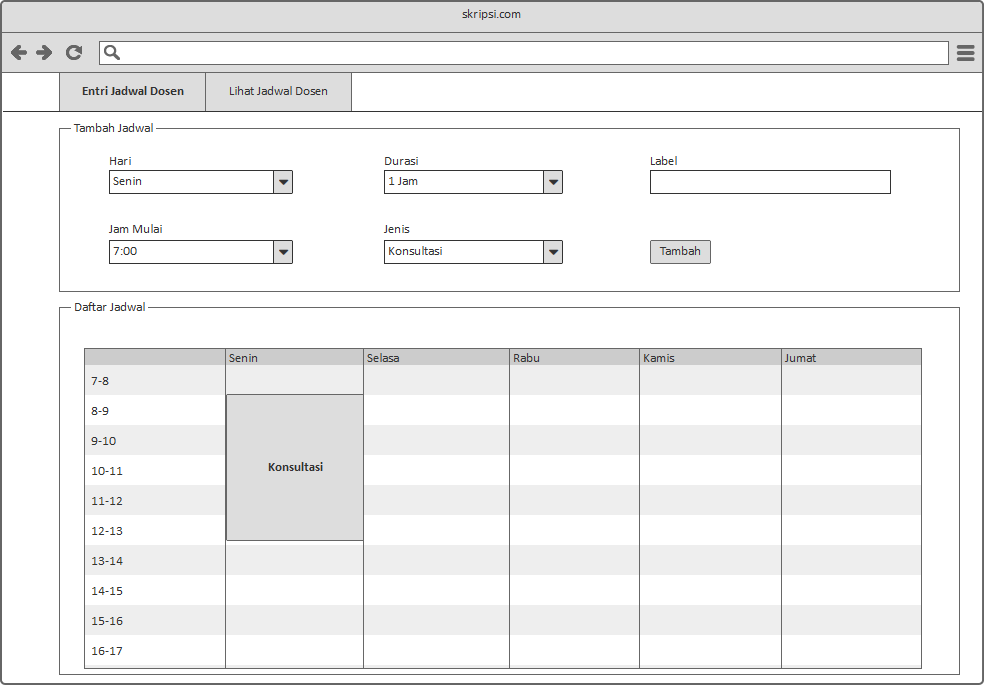
\includegraphics[scale=0.48]{entriJadwalDosen.png}
	\caption[Perancangan Antarmuka Entri Jadwal Dosen]{Perancangan Antarmuka Entri Jadwal Dosen} 
	\label{fig:flow-chart-CodeIgniter} 
\end{figure}
\subsection{Perancangan Antarmuka Edit Jadwal Dosen}
Perancangan antarmuka untuk \textit{pop-up} pengubahan data jadwal yang sudah dimasukan dapat dilihat pada gambar berikut
\begin{figure} [H]
	\centering  
	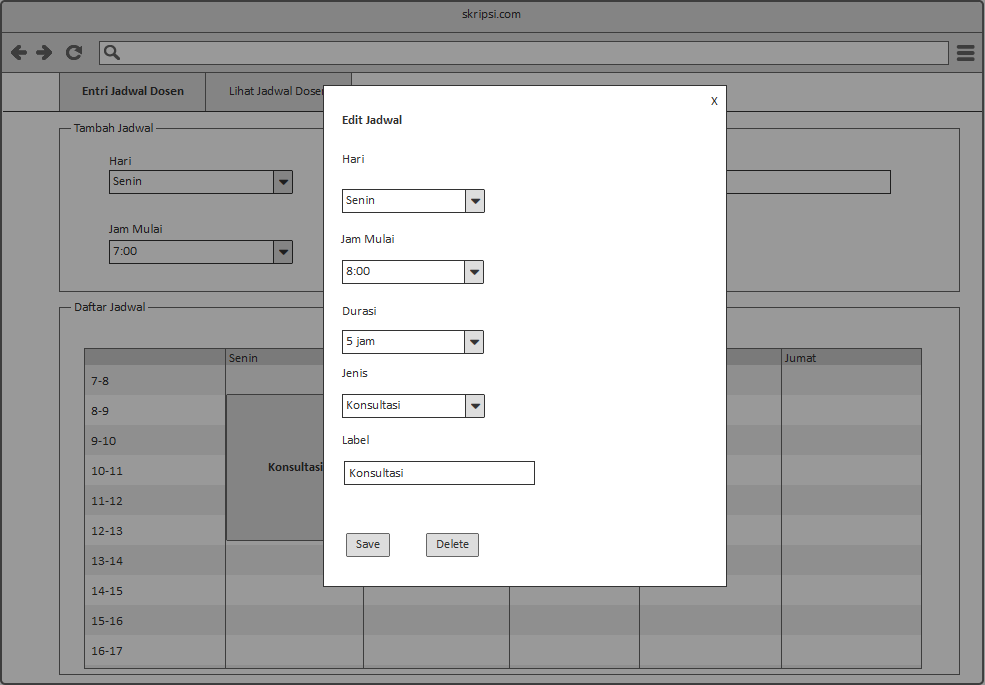
\includegraphics[scale=0.48]{editJadwalModal.png}
	\caption[Perancangan Antarmuka Edit Jadwal Dosen]{Perancangan Antarmuka Edit Jadwal Dosen} 
	\label{fig:flow-chart-CodeIgniter} 
\end{figure}
\subsection{Perancangan Antarmuka Lihat Jadwal Dosen}
Perancangan antarmuka untuk modul Lihat Jadwal Dosen dapat dilihat pada gambar di bawah ini
\begin{figure} [H]
	\centering  
	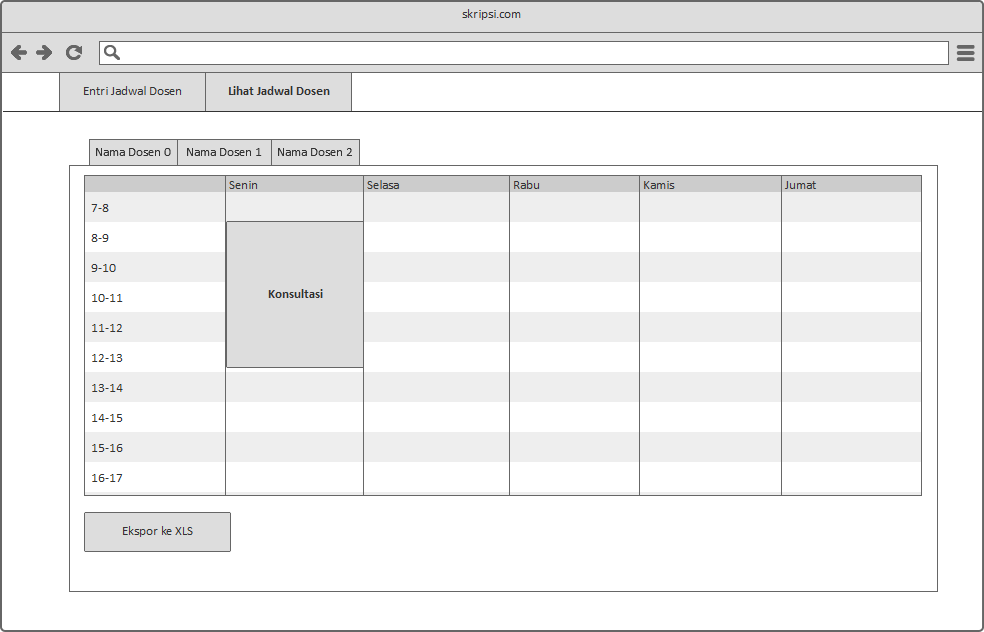
\includegraphics[scale=0.45]{lihatJadwalDosen.png}
	\caption[Perancangan Antarmuka Lihat Jadwal Dosen]{Perancangan Antarmuka Lihat Jadwal Dosen} 
	\label{fig:flow-chart-CodeIgniter} 
\end{figure}}{}
\ifdefstring{\vbabe}{1}{\lstset{
  basicstyle=\ttfamily,
  columns=fullflexible,
  frame=single,
  breaklines=true,
  postbreak=\mbox{\textcolor{red}{$\hookrightarrow$}\space},
}
\chapter{Implementasi dan Pengujian}
\label{chap:implementasiDanPengujian}
\setcounter{secnumdepth}{3}

\section{Implementasi}
\subsubsection{Lingkungan Pengembangan dan Pengujian Fungsional}
\paragraph{} Pembangunan perangkat lunak ini memakai bahasa pemrogaraman server PHP 5 dan MySQL 5.0 sebagai basis datanya. Pengembangan perangkat lunak ini dilakukan di komputer dengan spesifikasi perangkat keras dan perangkat lunaknya sebagai berikut:
\begin{itemize}
\item \textbf{Perangkat Keras}
\begin{enumerate}
	\item Prosesor AMD A6 VISION
	\item RAM 4 GB
	\item 500 GB harddisk
	\item Monitor
	\item Keyboard
	\item Mouse
\end{enumerate}
\item \textbf{Perangkat Lunak}
\begin{enumerate}
	\item Sistem Operasi Windows 8
	\item NetBeans IDE 8.0.2
	\item Server phpMyAdmin 4.3.11
	\item XAMPP Control Panel v3.2.1
	\item Client: Google Chrome 61.0.3163.100 32-bit
	\item Microsoft Excel 2013
\end{enumerate}

\end{itemize}
\subsection{Implementasi Basis Data}
\paragraph{}Implementasi basis data dalam Aplikasi Pembangkit Jadwal Dosen menggunakan satu tabel basis data. Tabel tersebut adalah tabel jadwal\_dosen yang menyimpan informasi-informasi seperti:
\begin{enumerate}
	\item user yang memiliki jadwal terkait
	\item hari berlangsungnya jadwal
	\item jam dimulainya kegiatan jadwal 
	\item durasi (dalam jam) lama berlangsungya jadwal
	\item nama kegiatan jadwal
	\item waktu terakhir jadwal diupdate
\end{enumerate}

\subsection{Implementasi Kelas}
Implementasi kelas dalam Aplikasi Pembangkit Jadwal Dosen terdiri dari kelas - kelas sebagai berikut:
\begin{enumerate}
	\item Kelas \textit{controller} EntriJadwalDosen\\
	Merupakan kelas yang mengatur hubungan antara kelas view EntriJadwalDosen dan kelas model JadwalDosen\_model.
	\item Kelas \textit{controller} LihatJadwalDosen\\
	Merupakan kelas yang berfungsi menghubungkan antara kelas view LihatJadwalDosen dan kelas model JadwalDosen\_model.
	\item Kelas \textit{view} EntriJadwalDosen yang berfungsi membuat \textit{user interface} untuk memasukan jadwal
	\item Kelas \textit{view} LihatJadwalDosen yang berfungsi membuat \textit{user interface} untuk memlihat jadwal
	\item Kelas model JadwalDosen\_model yang berfungsi untuk menulis atau membaca ke basis data.
\end{enumerate}

\section{Pengujian}
\paragraph{} Pengujian aplikasi ini dilakukan dengan menggunakan metode pengujian \textit{Black-Box Testing}. Pengujian ini difokuskan pada pengujian fungsional. Maksud dari pengujian fungsional ini adalah untuk menguji reaksi perangkat lunak terhadap aksi yang dilakukan oleh pengguna. Bila reaksi sistem tidak sesuai yang diharapkan, maka aplikasi masih memilki kekurangan.

\subsection{Pengujian Fungsional}
\subsubsection{Pengujian Fungsional Login}
Hasil pengujian dapat dilihat pada Tabel 5.1
\begin{center}
	\begin{table}[H]
		\begin{tabular}{|p{5cm}|p{5cm}|p{5cm}|}
		\hline
		\centering Aksi	& 	\centering Reaksi yang diharapkan &  \multicolumn{1}{c|}{Reaksi PL} \\
		\hline
		Menekan tombol login & Menampilkan menu login & Menampilkan menu login \\
		\hline
		\end{tabular}
		\caption{Pengujian Login}
	\end{table}
\end{center}

\subsubsection{Pengujian Fungsional Entri Jadwal Dosen}
Hasil pengujian dapat dilihat pada Tabel 5.2
\begin{center}
	\begin{table}[H]
		\begin{tabular}{|p{5cm}|p{5cm}|p{5cm}|}
		\hline
		\centering Aksi	& 	\centering Reaksi yang diharapkan &  \multicolumn{1}{c|}{Reaksi PL} \\
		\hline
		Memasukan data-data yang diperlukan untuk input jadwal & Jadwal yang sudah dimasukan muncul pada halaman Entri Jadwal Dosen & Jadwal yang sudah dimasukan muncul pada halaman Entri Jadwal Dosen \\
		\hline
		Data jadwal yang dimasukan tidak lengkap & Jadwal dimasukan dengan data yang sesuai nilai \textit{default} yang ditampilkan di menu & Jadwal dimasukan dengan data yang sesuai nilai \textit{default} yang ditampilkan di menu \\
		\hline
		Waktu dimulainya jadwal baru sama dengan jadwal yang sudah pernah dimasukan sebelumnya & Menampilkan pesan kesalahan dan batal memasukan data ke dalam database & Jadwal masuk ke dalam database, namun tidak muncul di halaman Entri Jadwal Dosen maupun halaman Lihat Jadwal Dosen \\
		\hline
		\end{tabular}
		\caption{Pengujian Fungsional Entri Jadwal Dosen}
	\end{table}
\end{center}

\subsubsection{Pengujian Fungsional Edit Jadwal Dosen}
Hasil pengujian dapat dilihat pada Tabel 5.3
\begin{center}
	\begin{table}[H]
		\begin{tabular}{|p{5cm}|p{5cm}|p{5cm}|}
		\hline
		\centering Aksi	& 	\centering Reaksi yang diharapkan &  \multicolumn{1}{c|}{Reaksi PL} \\
		\hline
		Memilih jadwal yang akan diedit & Memunculkan modal yang berisi menu edit yang menampilkan data-data jadwal yang sedang dipilih tersebut. Data-data tersebut juga dapat diubah oleh pengguna sesuai kebutuhannya & Memunculkan modal yang berisi menu edit yang menampilkan data-data jadwal yang sedang dipilih tersebut. Data-data tersebut juga dapat diubah oleh pengguna sesuai kebutuhannya \\
		\hline
		Memilih tombol simpan & Modal ditutup , data jadwal di \textit{database} diupdate sesuai dengan input user dan menampilkan menu Entri Jadwal Dosen & Modal ditutup , data jadwal di \textit{database} diupdate sesuai dengan input user dan menampilkan menu Entri Jadwal \\
		\hline
		Memilih tombol keluar & Modal ditutup lalu menampilkan menu Entri Jadwal Dosen & Modal ditutup lalu menampilkan menu Entri Jadwal Dosen \\
		\hline
		\end{tabular}
		\caption{Pengujian Fungsional Edit Jadwal Dosen}
	\end{table}
\end{center}

\subsubsection{Pengujian Fungsional Hapus Jadwal Dosen}
Hasil pengujian dapat dilihat pada Tabel 5.4
\begin{center}
	\begin{table}[H]
		\begin{tabular}{|p{5cm}|p{5cm}|p{5cm}|}
		\hline
		\centering Aksi	& 	\centering Reaksi yang diharapkan &  \multicolumn{1}{c|}{Reaksi PL} \\
		\hline
		Memilih jadwal yang akan diedit & Memunculkan modal yang berisi menu edit yang menampilkan data-data jadwal yang sedang dipilih tersebut. Data-data tersebut juga dapat diubah oleh pengguna sesuai kebutuhannya & Memunculkan modal yang berisi menu edit yang menampilkan data-data jadwal yang sedang dipilih tersebut. Data-data tersebut juga dapat diubah oleh pengguna sesuai kebutuhannya \\
		\hline
		Memilih tombol hapus & Modal ditutup dan jadwal dihapus dari basis data, lalu sistem menampilkan menu Entri Jadwal Dosen & Modal ditutup dan jadwal dihapus dari basis data, lalu sistem menampilkan menu Entri Jadwal Dosen \\
		\hline
		Memilih tombol keluar & Modal ditutup lalu menampilkan menu Entri Jadwal Dosen & Modal ditutup lalu menampilkan menu Entri Jadwal Dosen \\
		\hline
		\end{tabular}
		\caption{Pengujian Fungsional Hapus Jadwal Dosen}
	\end{table}
\end{center}

\subsubsection{Pengujian Fungsional Lihat Jadwal Dosen}
Hasil pengujian dapat dilihat pada Tabel 5.5
\begin{center}
	\begin{table}[H]
		\begin{tabular}{|p{5cm}|p{5cm}|p{5cm}|}
		\hline
		\centering Aksi	& 	\centering Reaksi yang diharapkan &  \multicolumn{1}{c|}{Reaksi PL} \\
		\hline
		Menekan tombol Lihat Jadwal Dosen & 
		Sistem menampilkan semua jadwal dosen dan mengelompokannya ke dalam tab-tab berdasarkan email setiap pemilik jadwal terkait. Kemudian setiap tab diberi label berisi nama lengkap pemilik jadwal tersebut. &
		Sistem menampilkan semua jadwal dosen dan mengelompokannya ke dalam tab-tab berdasarkan email setiap pemilik jadwal terkait. Kemudian setiap tab diberi label berisi nama lengkap pemilik jadwal tersebut.\\
		\hline
		\end{tabular}
		\caption{Pengujian Fungsional Lihat Jadwal Dosen}
	\end{table}
\end{center}

\subsubsection{Pengujian Fungsional Ekspor ke XLS}
Hasil pengujian dapat dilihat pada Tabel 5.6
\begin{center}
	\begin{table}[H]
		\begin{tabular}{|p{5cm}|p{5cm}|p{5cm}|}
		\hline
		\centering Aksi	& 	\centering Reaksi yang diharapkan &  \multicolumn{1}{c|}{Reaksi PL} \\
		\hline
		Menekan tombol ekspor ke XLS & 
		Sistem membuat file .xlsx yang berisi seluruh jadwal dosen yang dikelompokan ke dalam \textit{worksheet-worksheet} berdasarkan \textit{email} pemilik jadwal, lalu sistem  menampilkan menu untuk memilih lokasi penyimpanan file .xlsx yang akan diekspor ke komputer pengguna. &
		Sistem membuat file .xlsx yang berisi seluruh jadwal dosen yang dikelompokan ke dalam \textit{worksheet-worksheet} berdasarkan \textit{email} pemilik jadwal, lalu sistem  menampilkan menu untuk memilih lokasi penyimpanan file .xlsx yang akan diekspor ke komputer pengguna. \\
		\hline
		\end{tabular}
		\caption{Pengujian Fungsional Ekspor ke XLS}
	\end{table}
\end{center}


\section{Penugjian Ekperimental}
\paragraph{}Pengujian eksperimtal dilakukan dengan cara mengunggah kode-kode program ke bluetape.azure yang sudah digunakan oleh mahasiswa dan staf UNPAR sehingga dosen dapat memakai fasilitas baru ini untuk didapatkan. Pengujian ini dilakukan pada semester ganjil 2017/2018.Dari hasil pemakaian, didapatkan masukan-masukan dari pengguna aplkasi ini yang menjadi basis pengujian eksperimental.
Masukan-masukan ini disimpan ke dalam \textit{issue} git proyek BlueTape yang memiliki \textit{tag} "Jadwal Dosen". Semua \textit{issue} dapat dilihat di \textit{https://github.com/ftisunpar/BlueTape}.

\subsection{Pengujian Eksperimental Pembuatan File Spreadsheet Menggunakan Tipe Extensi File .xlsx}
\subsubsection{Permasalahan}
Pengujian ini merupakan hasil masukan dari Ibu Mariskha yang memilki masalah bahwa tab jadwal milik beliau tidak muncul setelah jadwal-jadwal diekspor ke dalam \textit{spreadsheet}.Pengujian ini dilakukan dengan mengekspor jadwal ke dalam tipe file .xlsx yang sudah digunakan sejak Microsoft Excel 2007.
\subsubsection{Analisis}
Ketika file .xlsx tersebut dibuka menggunakan Microsoft Excel 2013, muncul eror yang dapat dilihat pada Gambar 5.1 dan Gambar 5.2.
\begin{figure} [H]
	\centering  
	\frame{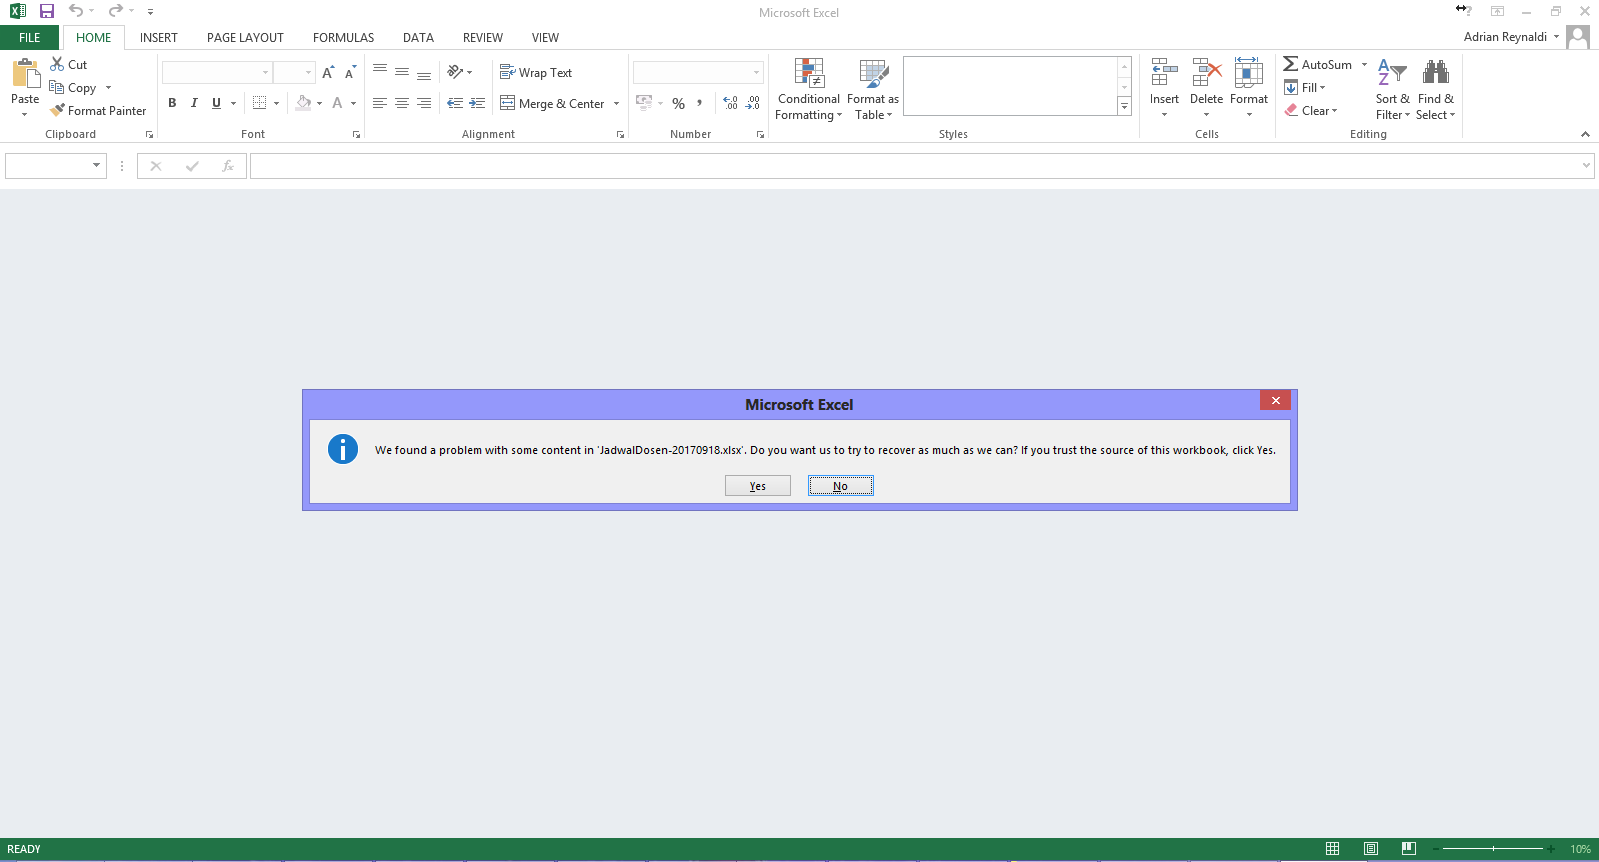
\includegraphics[scale=0.4]{erorXLSX.png}}
	\caption[Tampilan eror saat membuka file bertipe .xlsx]{Tampilan eror saat membuka file bertipe .xlsx} 
	\label{fig:flow-chart-CodeIgniter} 
\end{figure}

\begin{figure} [H]
	\centering  
	\frame{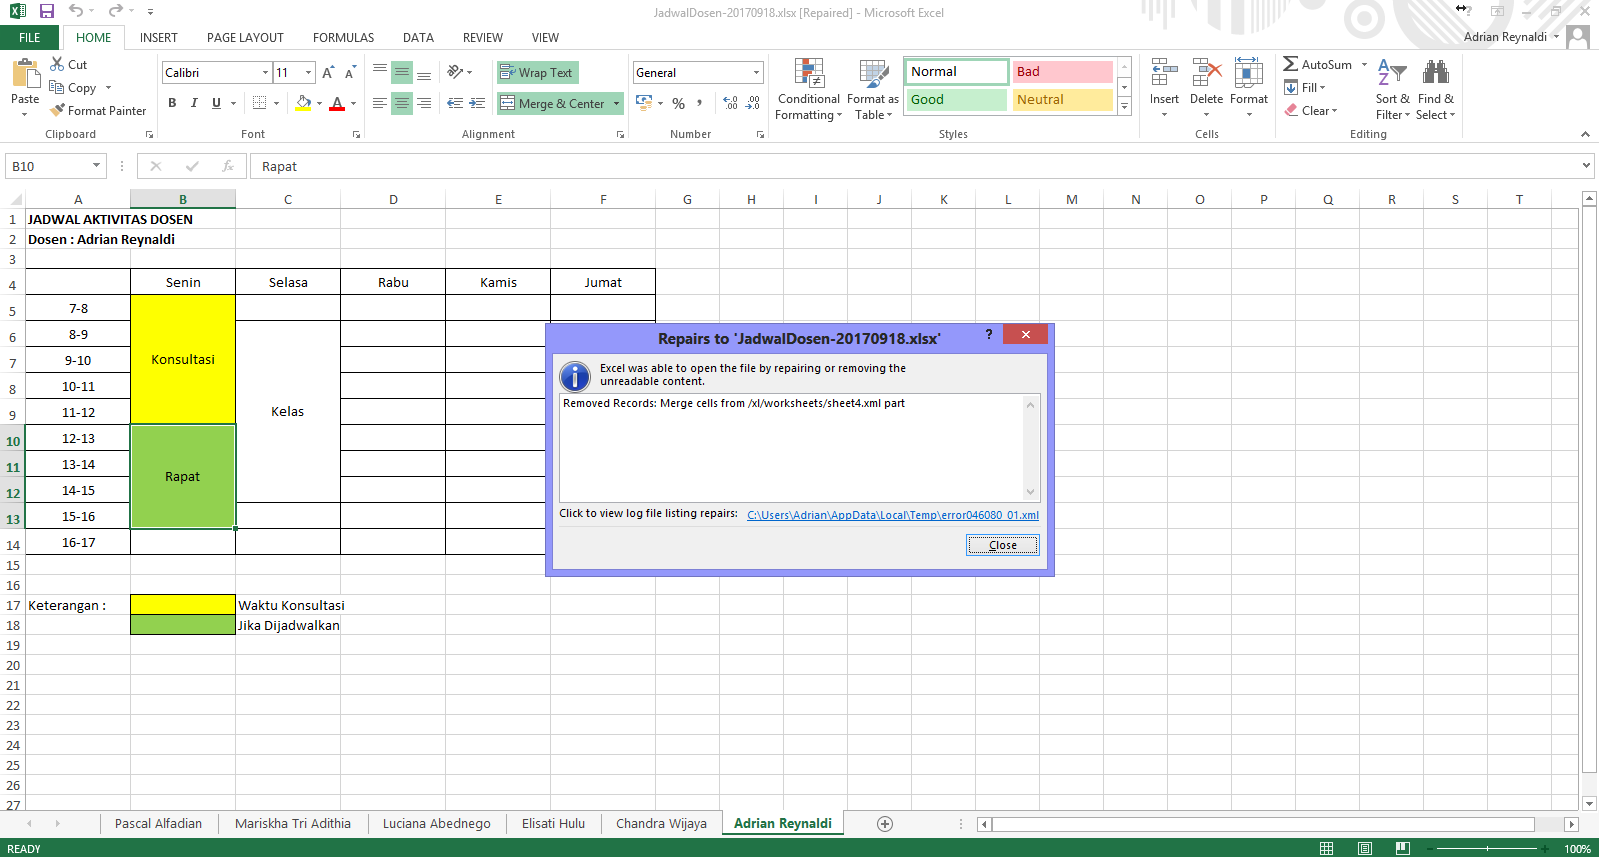
\includegraphics[scale=0.4]{erorXLSXDetail.png}}
	\caption[Keterangan Eror File .xlsx]{Keterangan Eror File .xlsx} 
	\label{fig:flow-chart-CodeIgniter} 
\end{figure}

Log eror:
\begin{lstlisting}
<?xml version="1.0" encoding="UTF-8" standalone="yes"?>
<recoveryLog xmlns="http://schemas.openxmlformats.org/spreadsheetml/2006/main">
<logFileName>error046080_01.xml</logFileName>
<summary>Errors were detected in file 'C:\Users\Adrian\Documents\Tugas\Skripsi\XLS Testing\JadwalDosen-20170918.xlsx'</summary>
<removedRecords summary="Following is a list of removed records:"><removedRecord>Removed Records: Merge cells from /xl/worksheets/sheet4.xml part
</removedRecord></removedRecords></recoveryLog>
\end{lstlisting}

\subsubsection{Hasil Pengujian dan Penyelesaian Masalah} 
\paragraph{}Dilihat dari log eror pada bagian Analisis di atas, eror terjadi karena ada perintah \textit{merge cells} yang dihapus oleh MS Excel. Hal ini terjadi karena adanya perintah dari PHPExcel versi 1.8.0 yang belum mendukung file bertipe .xlsx sehingga tab jadwal milik ibu Mariskha tidak muncul. Maka karena eror disebabkan oleh permasalahan kompabilitas PHPExcel 1.8.0 dan tipe file .xlsx,  hal ini dapat diatasi dengan cara mengubah tipe file yang diekspor dari file .xlsx menjadi tipe yang lebih lama yaitu .xls.
\newline
\newline
Potongan kode lama yang menyebabkan eror:
\begin{lstlisting}[caption={Kode Lama},captionpos=b]
 $filename = 'JadwalDosen-'.date("Ymd").'.xlsx'; //Nama file XLS yang akan dibuat
 header('Content-type: application/vnd.ms-excel');
 header('Content-Disposition: attachment;filename="' . $filename . '"');

 $objWriter = PHPExcel_IOFactory::createWriter($this->excel, 'Excel2007');
\end{lstlisting}
Potongan kode baru untuk menghilangkan eror:
\begin{lstlisting}[caption={Kode Baru},captionpos=b]
 $filename = 'JadwalDosen-'.date("Ymd").'.xls'; //Nama file XLS yang akan dibuat
 header('Content-type: application/vnd.ms-excel');
 header('Content-Disposition: attachment;filename="' . $filename . '"');

 $objWriter = PHPExcel_IOFactory::createWriter($this->excel, 'Excel5');
\end{lstlisting}
Seperti bisa dilihat pada dua potongan kode program di atas, terjadi perubahan pada baris pertama kode dan baris terakhir kode. Pada baris pertama ekstensi file diubah dari .xlsx menjadi .xls. Pada baris terakhir tipe spreadsheet diubah dari 'Excel2007' menjadi 'Excel5'.
\paragraph{}Setelah tipe file diubah menjadi  .xls, eror di Microsoft Excel pun hilang.
\begin{figure} [H]
	\centering  
	\frame{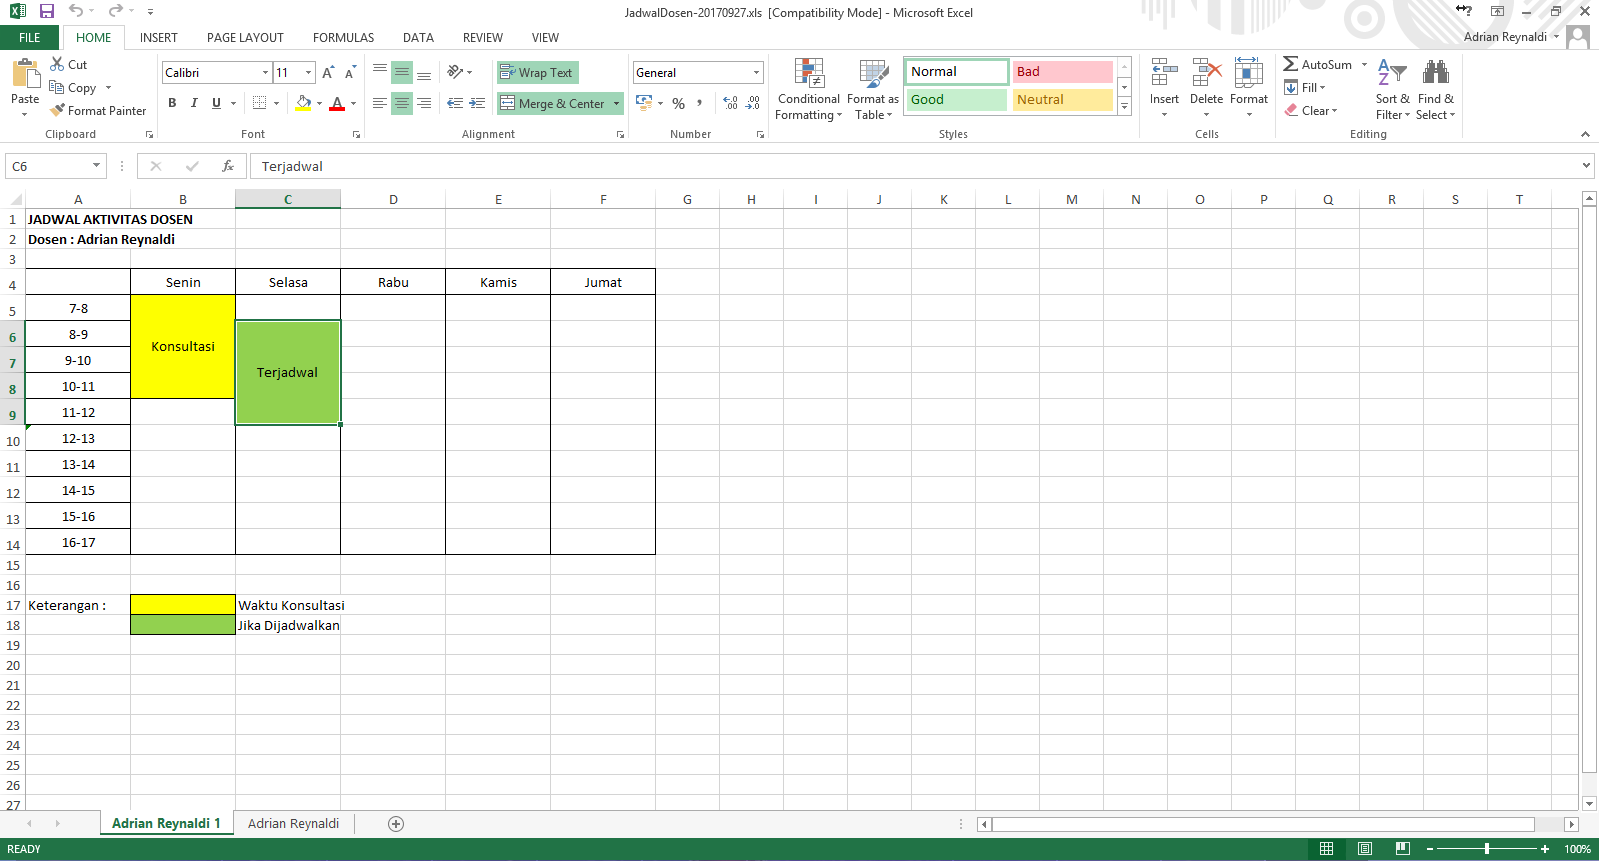
\includegraphics[scale=0.4]{tesXLSSukses.png}}
	\caption[Eror Sudah Tidak Muncul Ketika File Dibuka]{Eror Sudah Tidak Muncul Ketika File Dibuka} 
	\label{fig:eror-hilang} 
\end{figure}

\subsection{Pengujian Eksperimental Penambahan Tombol \textit{Delete All}}
\subsubsection{Masalah}
\paragraph{}Ketika jadwal yang dimasukan sudah sangat banyak, maka akan sulit untuk membersihkan tabel jadwal bila pengguna harus menghapus jadwal-jadwal tersebut satu per satu. Oleh karena itu Bapak Pascal mengusulkan untuk mengimplementasikan tombol "Delete All" yang berfungsi untuk menghapus semua jadwal yang sudah dimasukan oleh pengguna. 

\subsubsection{Analisis}
\paragraph{}Karena tombol "Delete All" ini memiliki pengaruh yang besar bila tidak sengaja tertekan oleh pengguna, maka diperlukan konfirmasi sebelum perintah penghapusan jadwal dieksekusi sistem.\newline
Untuk menangani itu diperlukan cara kerja sistem sebagai berikut:
\begin{enumerate}
	\item Ketika tombol "Delete All" ditekan akan ditampilkan \textit{pop-up} konfirmasi penghapusan jadwal.
	\item Lalu ketika tombol "ok" ditekan akan mengeksekusi perintah untuk menghapus semua jadwal milik user.
	\item Jika pengguna menekan tombol "cancel", sistem akan membatalkan perintah penghapusan jadwal dan menutup \textit{pop-up} konfirmasi.
\end{enumerate}
Untuk mengimplementasikan tombol "Delete All" diperlukan method tambahan pada controller EntriJadwalDosen dan JadwalDosen\_model untuk menghapus semua jadwal berdasarkan username/email pengguna..
\begin{center}
\begin{table}[H]
\begin{tabular}{|c|p{11cm}|}
\hline
Nama Method 	& 	deleteAll 	\\
\hline
Parameter Input & email via POST \\
\hline
Parameter Output & - \\
\hline
Tabel yang berhubungan & jadwal\_dosen \\
\hline
Deskripsi	& Proses untuk memanggil method pada model JadwalDosen\_model untuk menghapus semua jadwal milik pengguna \\
\hline
Algoritma	& \begin{itemize}
				\item proses menerima input berupa email pengguna.
				\item proses memanggil method deleteByUsername(email) dari kelas JadwalDosen\_model dengan parameter email diisi dengan nama email pengguna.
				\end{itemize} \\
\hline
\end{tabular}
\caption{Perancangan method deleteAll}
\end{table}
\end{center}

\begin{center}
\begin{table}[H]
\begin{tabular}{|c|p{11cm}|}
\hline
Nama Method 	& 	deleteByUsername 	\\
\hline
Parameter Input & email via POST \\
\hline
Parameter Output & - \\
\hline
Tabel yang berhubungan & jadwal\_dosen \\
\hline
Deskripsi	& Proses untuk menghapus semua jadwal milik pengguna di basis data\\
\hline
Algoritma	& \begin{itemize}
				\item proses menerima input berupa email dari controller EntriJadwalDosen.
				\item proses menghapus semua jadwal pengguna dari database.
				\end{itemize} \\
\hline
\end{tabular}
\caption{Perancangan method deleteByUsername}
\end{table}
\end{center}

\subsubsection{Hasil Pengujian dan Penyelesaian Masalah}
Tombol "Delete All" dibuat di halaman EntriJadwalDosen di pojok kiri bawah.
\begin{figure} [H]
	\centering  
	\frame{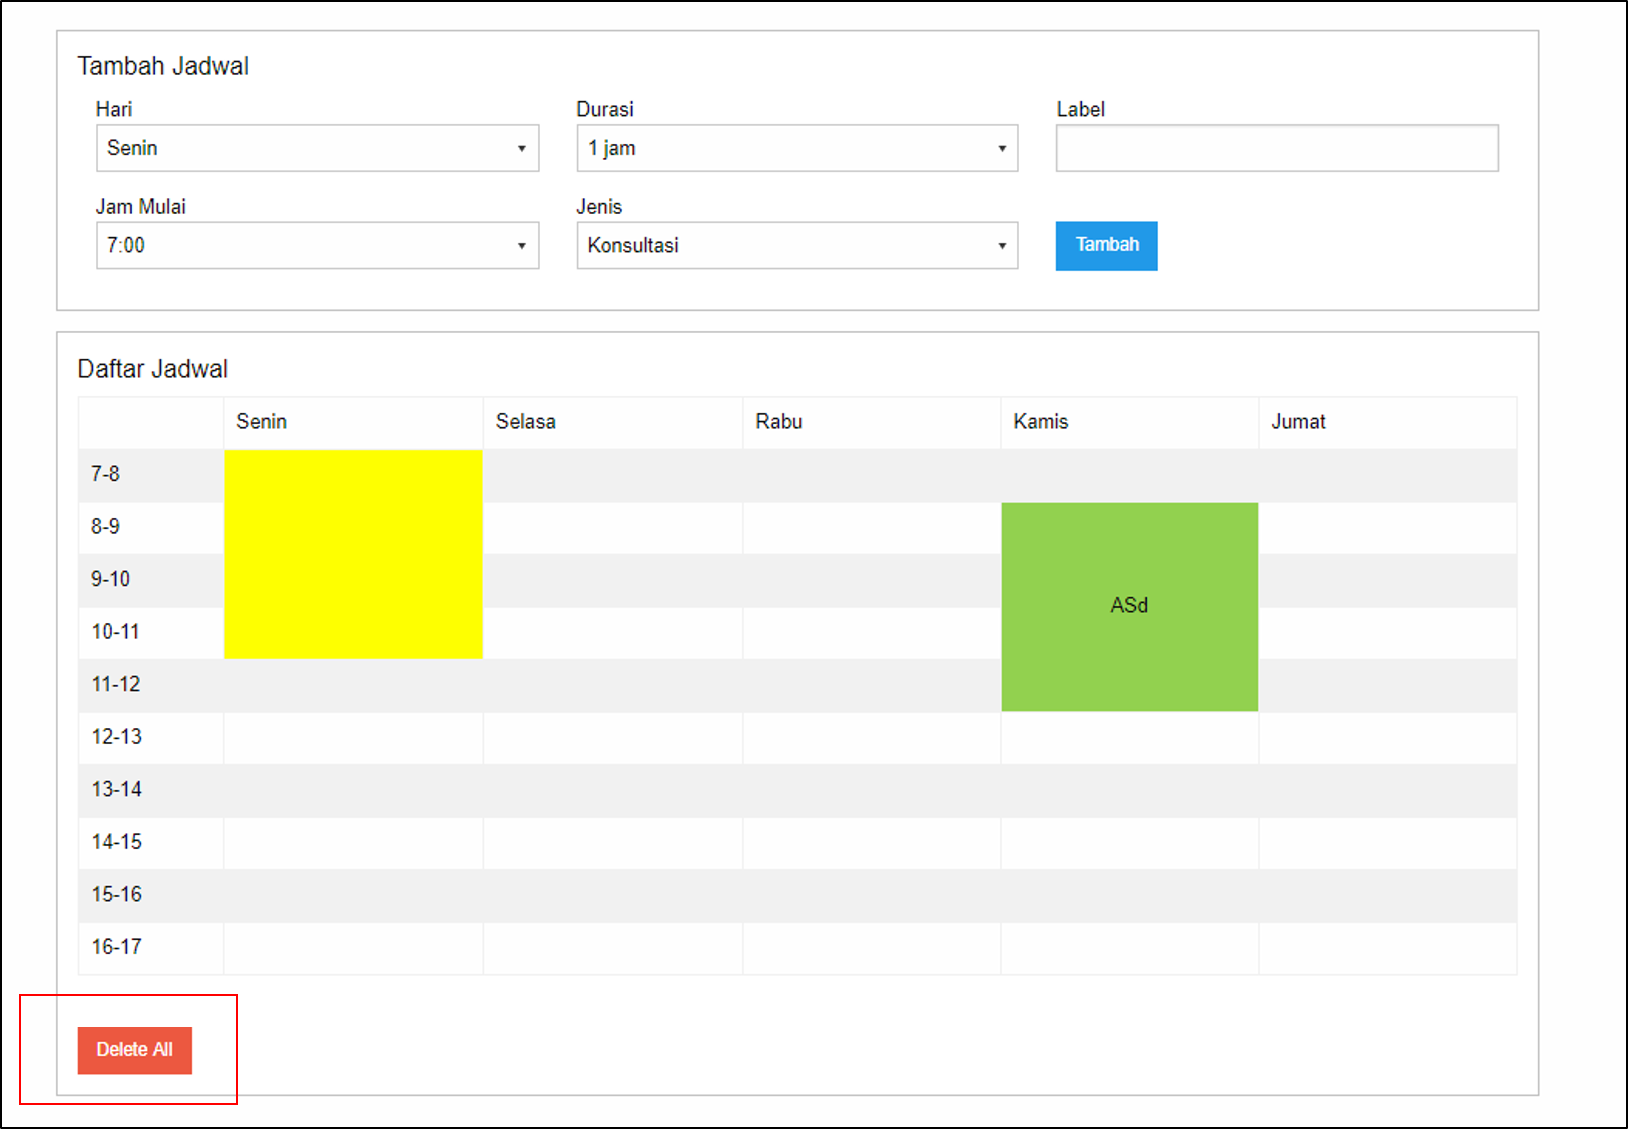
\includegraphics[scale=0.5]{deleteAllButton.png}}
	\caption[Tombol \textit{Delete All} di Entri Jadwal Dosen]{Tombol \textit{Delete All} di Entri Jadwal Dosen} 
	\label{fig:flow-chart-CodeIgniter} 
\end{figure}
Ketika tombol "Delete All" ditekan memunculkan tampilan konfirmasi
\begin{figure} [H]
	\centering  
	\frame{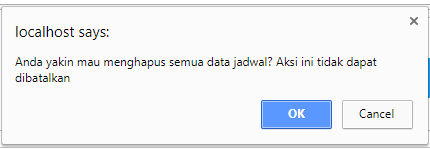
\includegraphics[scale=0.5]{popupDeleteAll.png}}
	\caption[Tampilan Konfirmasi]{\textbf{Tombol \textit{Delete All} di Entri Jadwal Dosen}} 
	\label{fig:flow-chart-CodeIgniter} 
\end{figure}
Setelah tombol "ok" ditekan, semua jadwal dihapus
\begin{figure} [H]
	\centering  
	\frame{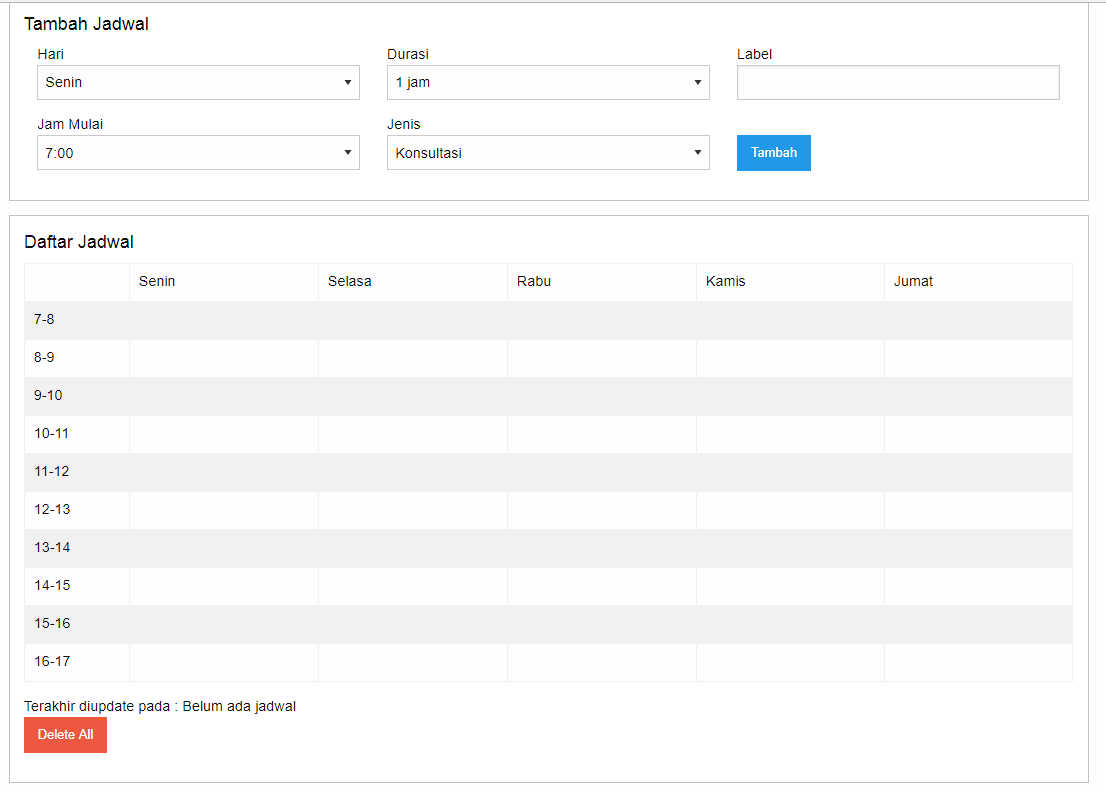
\includegraphics[scale=0.5]{empty.png}}
	\caption[Semua Jadwal Dihapus]{Semua Jadwal Dihapus} 
	\label{fig:flow-chart-CodeIgniter} 
\end{figure}
Hasil pengujian berjalan lancar dan sesuai dengan hasil yang diharapkan.

\subsection{Pengujian Eksperimental Penambahan Informasi Waktu \textit{Update} Terakhir Jadwal}
\subsubsection{Masalah}
\paragraph{}Fitur ini merupakan usulan dari Bapak Pascal karena sering kali pengguna lupa kapan terakhir kali pengguna memasukan atau mengubah jadwal. Hal ini menyulitkan pengguna untuk mengetahui apakah jadwal yang telah ia masukan dapat dipakai atau tidak.
\subsubsection{Analisis}
\paragraph{}Informasi waktu \textit{update} terakhir jadwal oleh pengguna berfungsi agar pengguna dapat membedakan apakah jadwal miliknya merupakan versi lama yang sudah tidak dipakai atau merupakan versi baru. Hasil yang diharapkan adalah muncul label di halaman EntriJadwalDosen dan LihatJadwalDosen.\\
Untuk mengimplementasikan fitur ini perlu ditambahkan field baru di tabel jadwal\_dosen:
\begin{center}
\begin{table}[h]
\begin{tabular}{|c|c|c|c|c|c|}
 			\hline
		\textbf{Atribut} & \textbf{Tipe Data} & \textbf{Ukuran} & \textbf{PK* / FK*}  & \textbf{Keterangan} \\
			\hline
		 lastUpdate & datetime & - & bukan PK/FK &  tanggal terakhir jadwal di-\textit{update}\\
		 \hline
	\end{tabular}
	\caption{Perancangan field tambahan di jadwal\_dosen}
	\end{table}
\end{center}
\subsubsection{Hasil Pengujian dan Penyelesaian Masalah}
Label yang bertuliskan informasi mengenai tanggal terakhir \textit{update} jadwal muncul di halaman EntriJadwalDosen
\begin{figure} [H]
	\centering  
	\frame{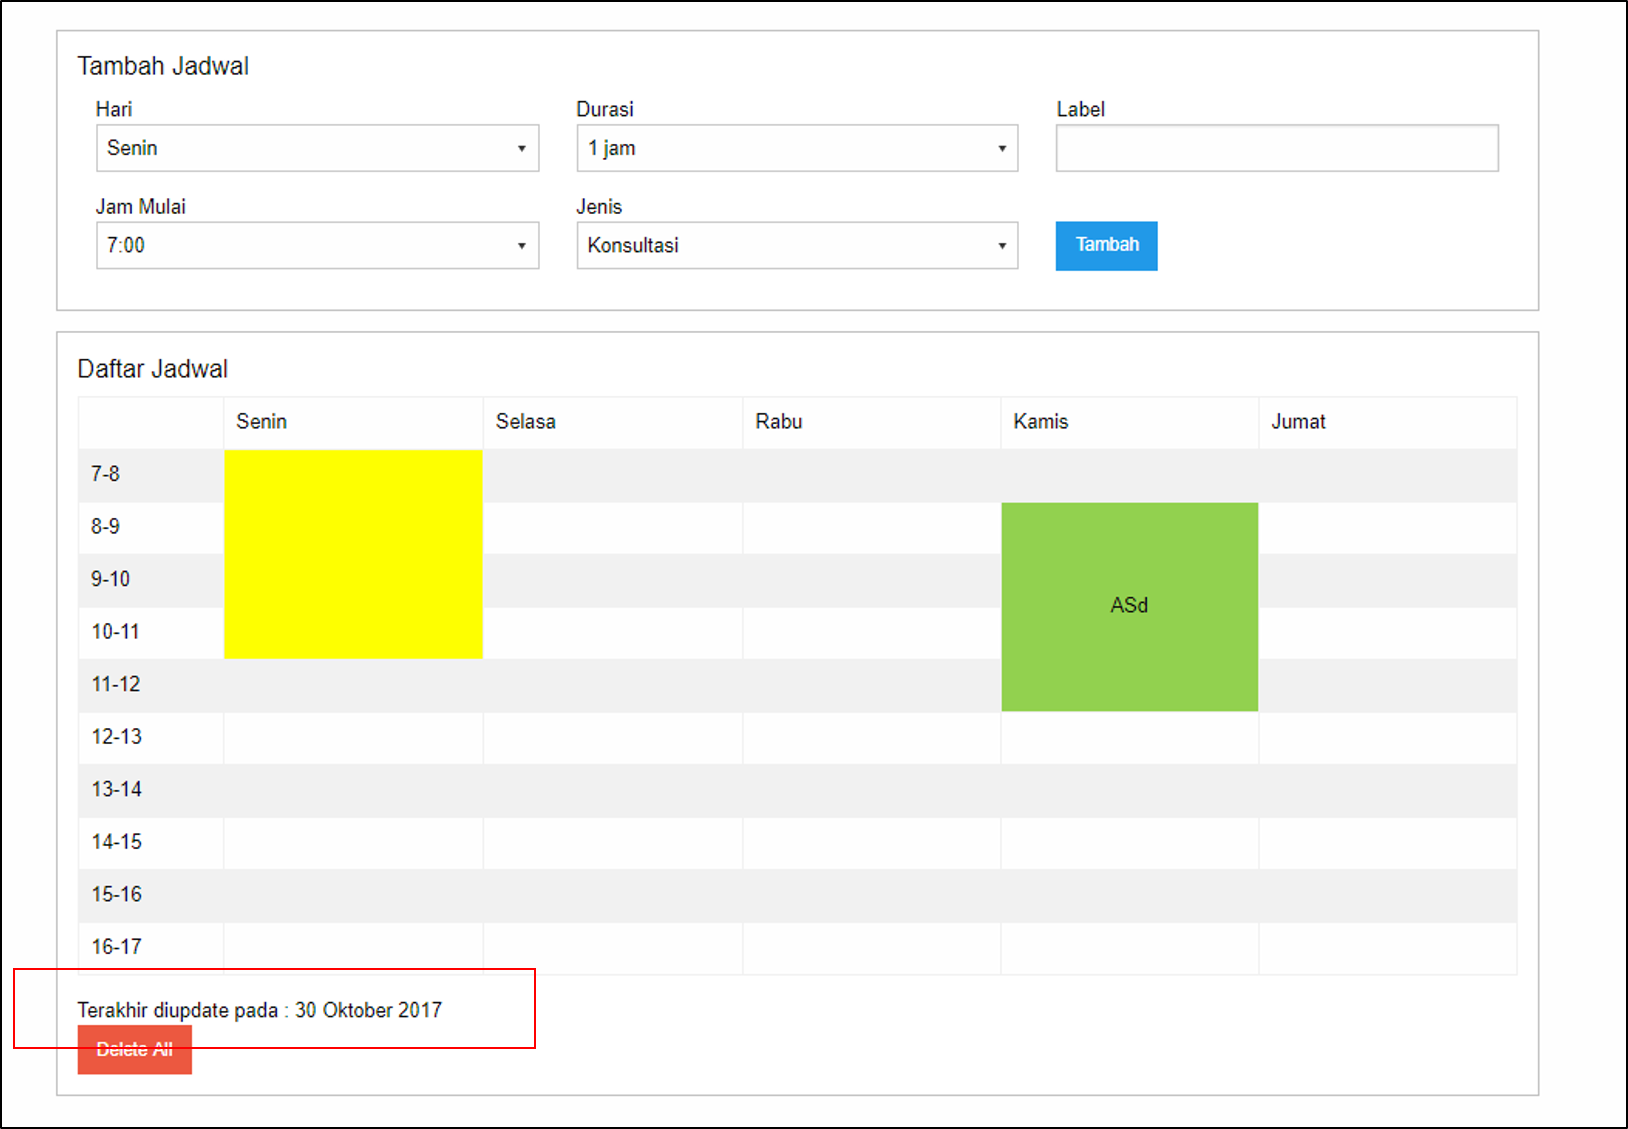
\includegraphics[scale=0.5]{updateTerakhir.png}}
	\caption[Informasi Waktu \textit{Update} Terakhir Jadwal di Entri Jadwal Dosen]{Informasi Waktu \textit{Update} Terakhir Jadwal di Entri Jadwal Dosen}
\end{figure}
Label berisi tanggal terakhir update jadwal muncul di halaman LihatJadwalDosen
\begin{figure} [H]
	\centering  
	\frame{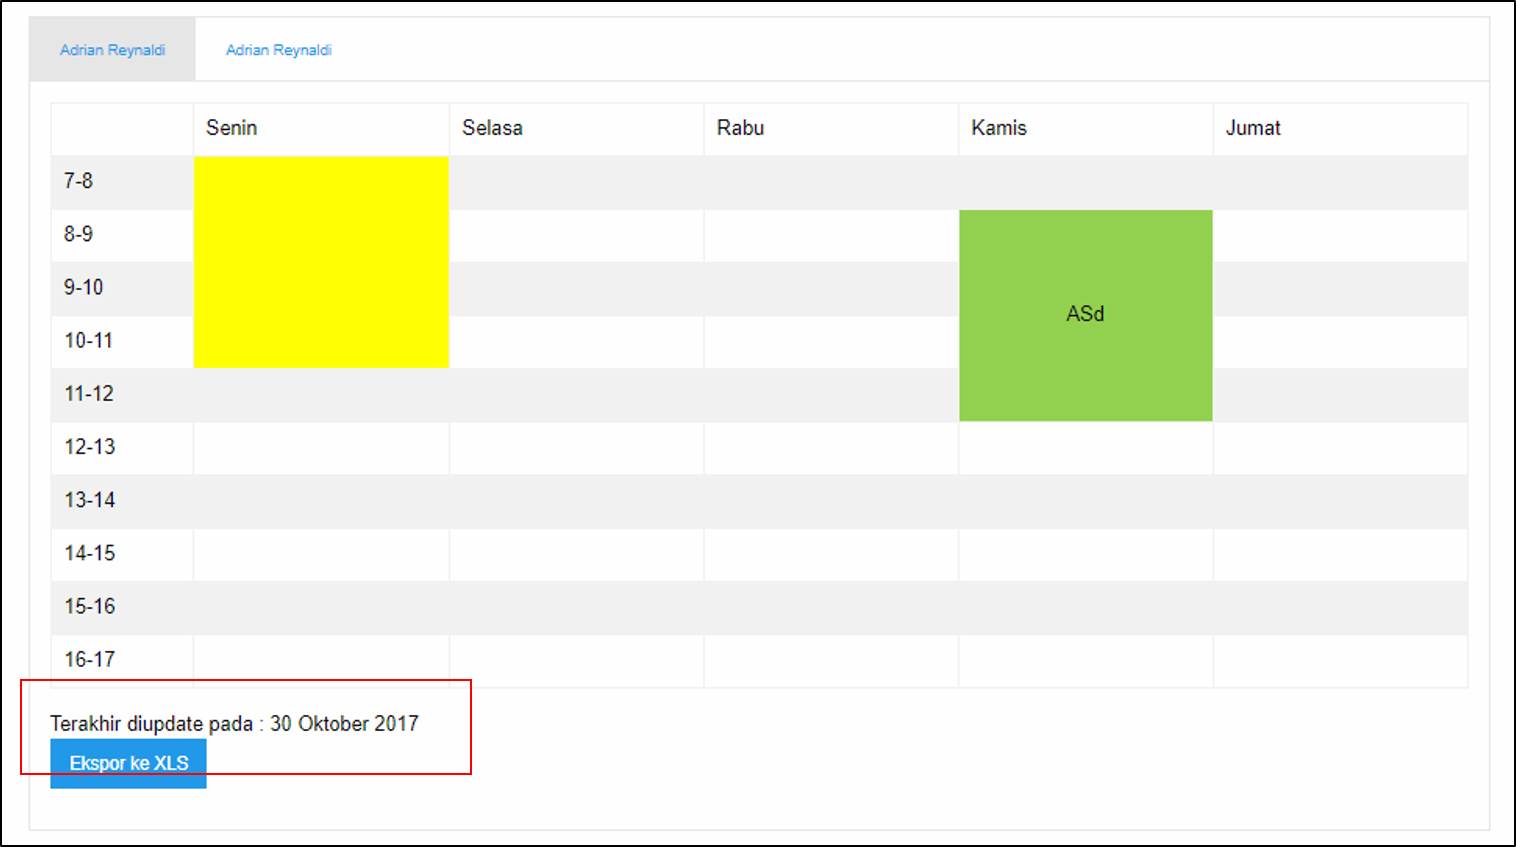
\includegraphics[scale=0.5]{updateTerakhirLihat.png}}
	\caption[Informasi Waktu \textit{Update} Terakhir Jadwal di Lihat Jadwal Dosen]{Informasi Waktu \textit{Update} Terakhir Jadwal di Lihat Jadwal Dosen}
\end{figure}
Hasil pengujian berjalan lancar dan sesuai dengan hasil yang diharapkan.

\subsection{Pengujian Eksperimental \textit{Conflict Handler}}
\subsubsection{Masalah}
\paragraph{}Terdapat masalah bila ketika pengguna memasukan atau mengupdate jadwal, sistem tidak memeriksa apakah sudah ada jadwal pada waktu yang dimasukan oleh pengguna. Masalah ini merupakan masalah yang ditemukan oleh penulis sendiri.
\subsubsection{Analisis}
Untuk mencegah pengguna memasukan jadwal yang akan menimbulkan konflik dengan jadwal yang sudah ada, maka sistem perlu memeriksa:
\begin{itemize}
	\item Memeriksa apakah sudah ada jadwal di jam mulai jadwal baru.
	\item Memeriksa apakah sudah ada jadwal di jam akhir jadwal baru.
\end{itemize}
Untuk mencegah pengguna juga kebingungan ketika sistem menolak memasukan jadwal karena terjadinya konflik, maka perlu adanya:
\begin{itemize}
	\item Tampilan eror bahwa jadwal baru gagal dimasukan karena terjadi bentrok dengan jadwal lama.
	\item Tampilan eror bahwa edit jadwal gagal dilakukan karena terjadi bentrok dengan jadwal lain.
\end{itemize}
\subsubsection{Hasil Pengujian dan Penyelesaian Masalah}
Terdapat dua pengujian, yaitu pengujian pertama untuk memeriksa apakah konflik ketika memasukan jadwal baru sudah tertangani. Lalu pengujian kedua untuk memeriksa apakah konflik ketika mengubah jadwal yang menyebabkan bentrok dengan jadwal lain sudah ditangani.
\begin{enumerate}
	\item \textbf{Pengujian Pertama}\\
	Mencoba memasukan jadwal di hari Selasa jam 7 pagi ketika sudah ada jadwal lain di jam dan hari tersebut.
\begin{figure} [H]
	\centering  
	\frame{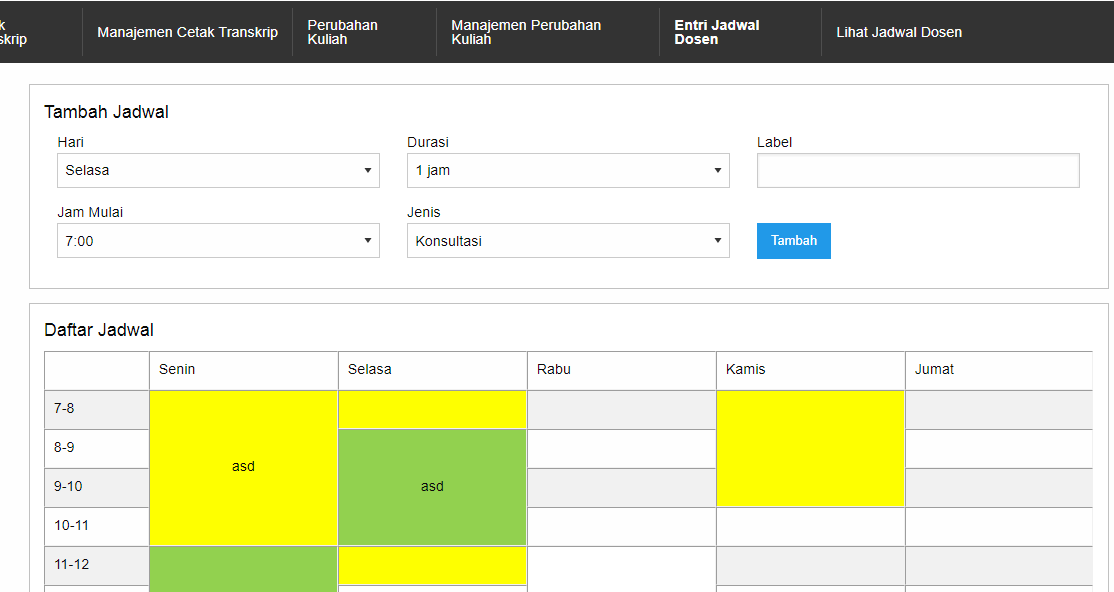
\includegraphics[scale=0.5]{memasukanBentrok.png}}
	\caption[Memasukan Jadwal ke Waktu yang Sudah Ada Jadwal]{Memasukan Jadwal ke Waktu yang Sudah Ada Jadwal} 
\end{figure}
	Muncul tampilan eror yang memberi tahu pengguna bahwa jadwal yang ingin dimasukan gagal masuk karena terjadi bentrok.
\begin{figure} [H]
	\centering  
	\frame{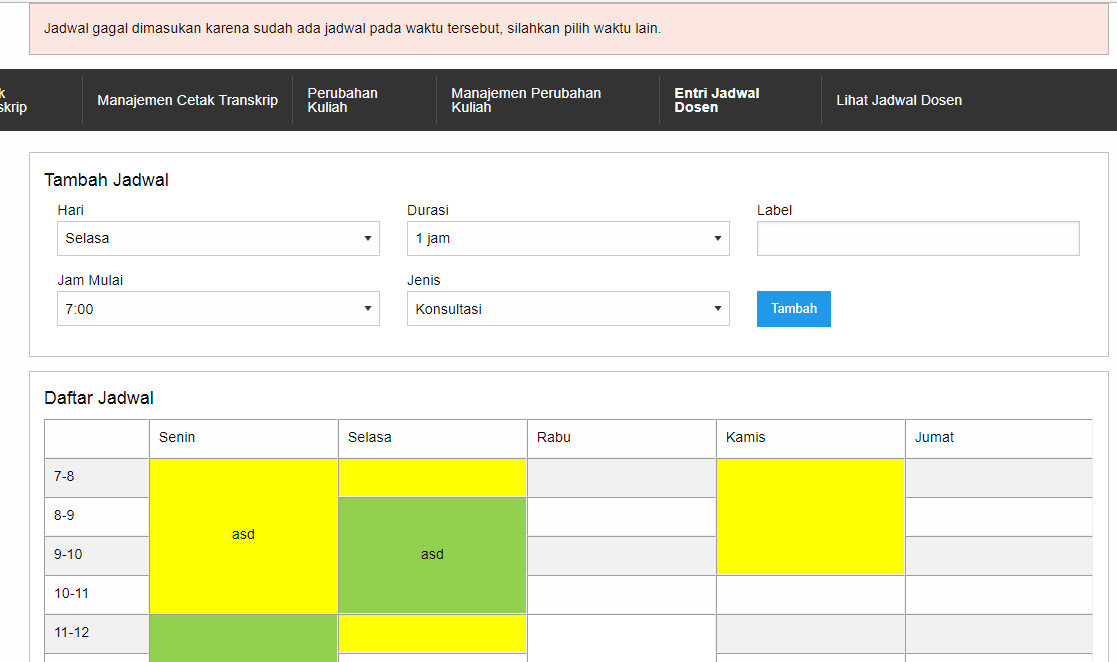
\includegraphics[scale=0.5]{GagalMasuk.png}}
	\caption[Tampilan Eror Gagal Masuk]{Tampilan Eror Gagal Masuk} 
\end{figure}

	\item \textbf{Pengujian Kedua}
	Daftar jadwal yang sudah ada dapat dilihat di Gambar 5.11
	\begin{figure} [H]
	\centering  
	\frame{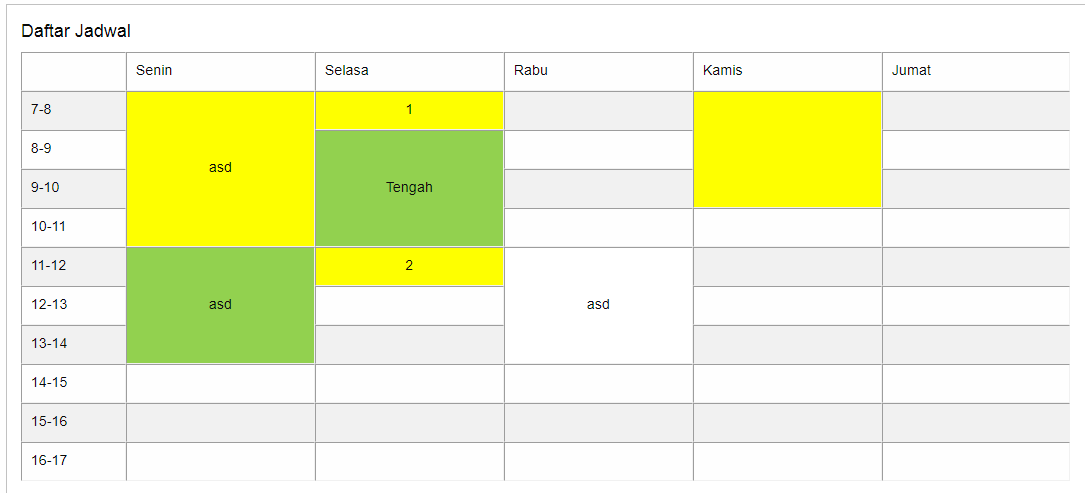
\includegraphics[scale=0.5]{daftarJadwal.png}}
	\caption[Jadwal yang Sudah Ada]{Jadwal yang Sudah Ada} 
	\end{figure}
	Mencoba mengubah jadwal "1" menjadi berdurasi 3 jam sehingga memicu bentrok dengan jadwal "Tengah".
	\begin{figure} [H]
	\centering  
	\frame{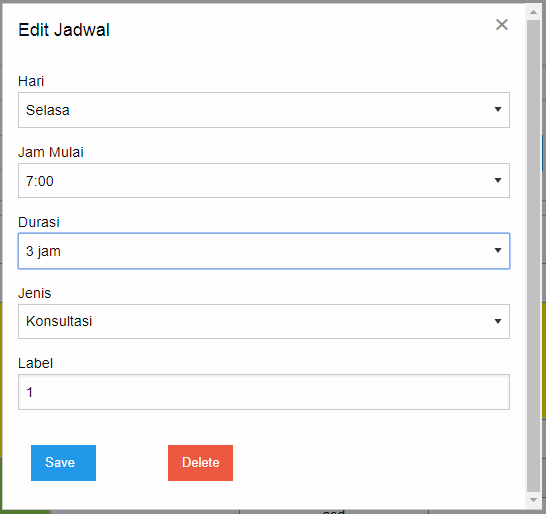
\includegraphics[scale=0.5]{mengeditBentrok.png}}
	\caption[Mengubah Jadwal "1"]{Mengubah Jadwal "1"} 
	\end{figure}
	Muncul tampilan eror yang memberi tahu bahwa jadwal gagal diubah.
	\begin{figure} [H]
	\centering  
	\frame{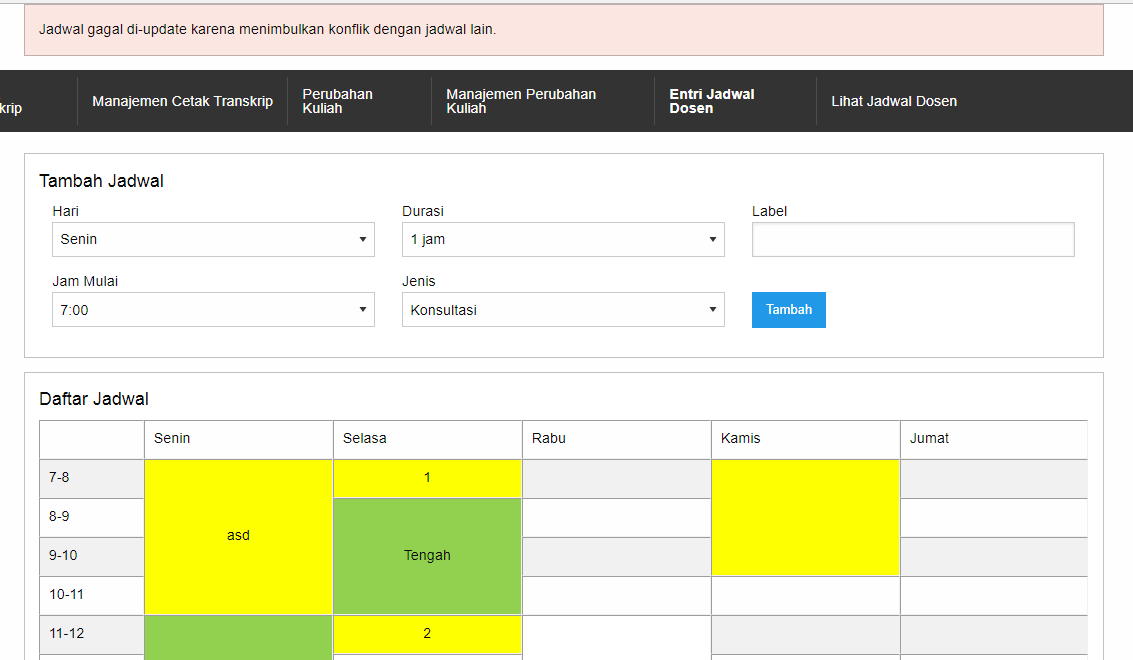
\includegraphics[scale=0.5]{gagalUpdate.png}}
	\caption[Tampilan Eror Gagal \textit{Update}]{Tampilan Eror Gagal \textit{Update}} 
	\end{figure}
	Mencoba mengubah jadwal "2" menjadi mulai pada jam 10 sehingga memicu bentrok dengan jadwal "Tengah".
	\begin{figure} [H]
	\centering  
	\frame{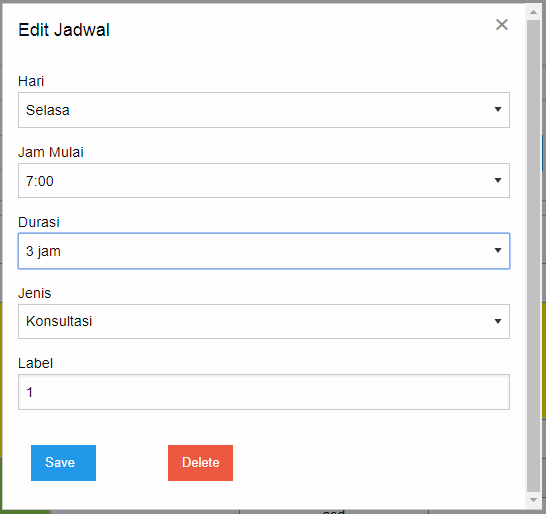
\includegraphics[scale=0.5]{mengeditBentrok.png}}
	\caption[Mengubah Jadwal "2"]{Mengubah Jadwal "2"} 
	\end{figure}
	Muncul tampilan eror yang memberi tahu bahwa jadwal gagal diubah.
	\begin{figure} [H]
	\centering  
	\frame{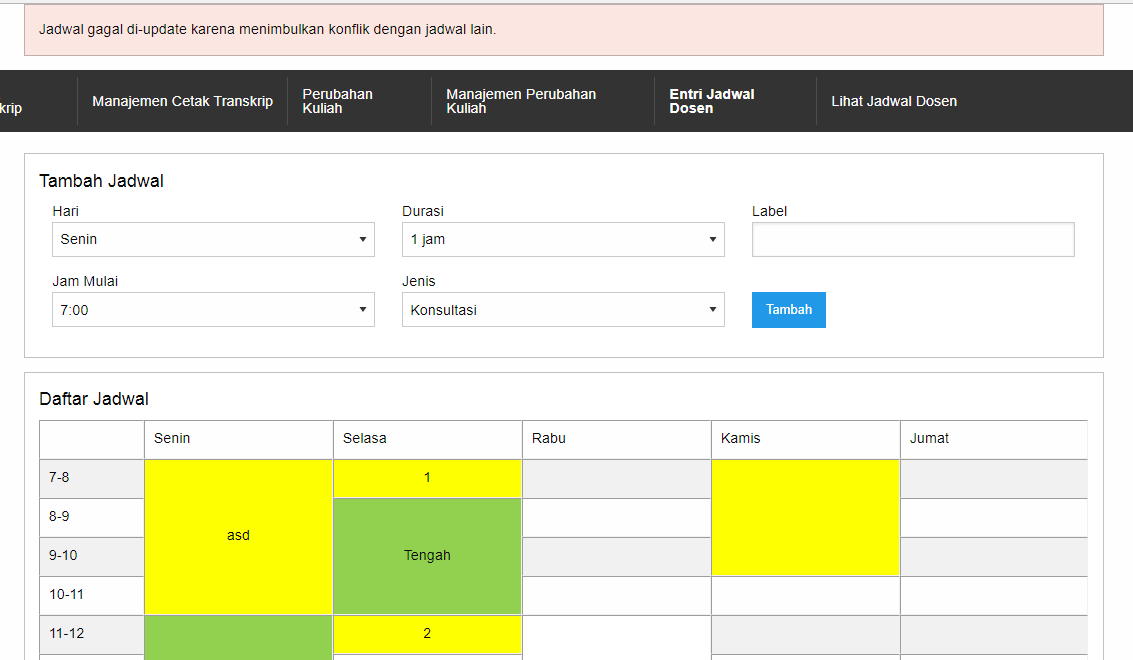
\includegraphics[scale=0.5]{gagalUpdate.png}}
	\caption[Tampilan Eror Gagal \textit{Update}]{Tampilan Eror Gagal \textit{Update}} 
	\end{figure}
\end{enumerate}
Setelah kedua pengujian di atas maka dapat disimpulkan pengujian berjalan dengan lancar dan hasil yang diharapkan tercapai.

}{}
\ifdefstring{\vbabf}{1}{\chapter{Kesimpulan dan Saran}
\section{Kesimpulan}
\paragraph{} Penelitian yang dilakukan dalam pengembangan Aplikasi Pembangkit Jadwal Dosen berhasil memenuhi harapan dalam mencatat dan menampilkan jadwal dosen. Kesimpulan yang dapat diambil dari hasil penelitian adalah sebagai berikut:
\begin{enumerate}
	\item Aplikasi memenuhi tujuan dalam mengotentikasi pengguna yang mengakses BlueTape. Pengguna dosen dapat mengakses modul Entri Jadwal Dosen dan Lihat Jadwal Dosen sedangkan pengguna mahasiswa hanya dapat mengakses modul Lihat Jadwal Dosen.
	\item Aplikasi memenuhi tujuan menyediakan cara bagi dosen untuk memasukan jadwalnya ke dalam BlueTape dengan mengimplementasikan modul Entri Jadwal Dosen yang berisi menu untuk menambah jadwal. Selain itu, aplikasi ini juga memenuhi tujuan agar jadwal dosen dapat ditampilkan di BlueTape dengan mengimplementasikan modul Lihat Jadwal Dosen yang menampilkan setiap jadwal dosen dalam bentuk tabel-tabel.
	\item Aplikasi memenuhi tujuan untuk mengekspor jadwal yang disimpan di basis data menjadi tipe file xls.
\end{enumerate}

\section{Saran}
\paragraph{}Berdasarkan hasil kesimpulan di atas, maka berikut merupakan saran-saran yang dapat diberikan untuk pengembangan selanjutnya:
\begin{enumerate}
	\item Ditemukan bahwa format email untuk mahasiswa angkatan 2017 memiliki format yang berbeda dengan mahasiswa-mahasiswa angkatan sebelumnya. Mahasiswa angkatan 2017 memiliki format xxxx73yyyy@student.unpar.ac.id xxxx merupakan angkatan dan yyyy merupakan nomor pokoknya. Sedangkan sebelumnya email mahasiswa memilki format 73xxyyyy@student.unpar.ac.id dengan xx adalah angkatan dan yyyy nomor pokoknya. Perlu dikaji ulang cara otentikasi dan pengelompokan pengguna mahasiswa pada penerapan Google OAuth.
	\item Mengurutkan tab-tab jadwal dosen berdasarkan alphabet atau urutan lainnya agar nama dosen mudah untuk dicari.
	\item Mengganti \textit{library} PHPExcel dengan versi terbarunya yaitu PHPOffice untuk mendukung pembuatan file bertipe .xlsx agar ukuran file lebih kecil.
\end{enumerate}
}{}
\ifdefstring{\vbabg}{1}{\include{Bab/bab7}}{}
\ifdefstring{\vbabh}{1}{\include{Bab/bab8}}{}
\ifdefstring{\vbabi}{1}{\include{Bab/bab9}}{}

\bibliographystyle{ieeetr}
\bibliography{pustaka}

\appendix
\apptoc

\tampillmp{\vlmp}
\ifdefstring{\vlmpa}{1}{%versi 3 (18-12-2016)
\chapter{Kode Program}
\label{lamp:A}

%terdapat 2 cara untuk memasukkan kode program
% 1. menggunakan perintah \lstinputlisting (kode program ditempatkan di folder yang sama dengan file ini)
% 2. menggunakan environment lstlisting (kode program dituliskan di dalam file ini)
% Perhatikan contoh yang diberikan!!
%
% untuk keduanya, ada parameter yang harus diisi:
% - language: bahasa dari kode program (pilihan: Java, C, C++, PHP, Matlab, C#, HTML, R, Python, SQL, dll)
% - caption: nama file dari kode program yang akan ditampilkan di dokumen akhir
%
% Perhatian: Abaikan warning tentang textasteriskcentered!!
%


\begin{lstlisting}[language=Java, caption=MyCode.c]

// This does not make algorithmic sense, 
// but it shows off significant programming characters.

#include<stdio.h>

void myFunction( int input, float* output ) {
	switch ( array[i] ) {
		case 1: // This is silly code
			if ( a >= 0 || b <= 3 && c != x )
				*output += 0.005 + 20050;
			char = 'g';
			b = 2^n + ~right_size - leftSize * MAX_SIZE;
			c = (--aaa + &daa) / (bbb++ - ccc % 2 );
			strcpy(a,"hello $@?"); 
	}
	count = ~mask | 0x00FF00AA;
}

// Fonts for Displaying Program Code in LATEX
// Adrian P. Robson, nepsweb.co.uk
// 8 October 2012
// http://nepsweb.co.uk/docs/progfonts.pdf

\end{lstlisting}

\lstinputlisting[language=Java, caption=MyCode.java]{./Lampiran/MyCode.java} 

}{}
\ifdefstring{\vlmpb}{1}{%versi 2 (8-10-2016)
\chapter{Kode Program Implementasi Modul Lihat Jadwal Dosen}
\label{Implementasi Modul Lihat Jadwal Dosen}

Kode Program untuk \textit{controller} modul Lihat Jadwal Dosen
\lstinputlisting[language=php, caption=LihatJadwalDosen.php]{./Lampiran/LihatJadwalDosen.php} 

Kode Program untuk \textit{view} modul Lihat Jadwal Dosen
\lstinputlisting[language=php, caption=main.php]{./Lampiran/lihatJadwalDosenView.php} 

}{}
\ifdefstring{\vlmpc}{1}{%versi 2 (8-10-2016)
\chapter{Kode Program Model JadwalDosen}
\label{Implementasi Modul Lihat Jadwal Dosen}

Kode program untuk mengimplementasikan model JadwalDosen
\lstinputlisting[language=php, caption=JadwalDosen\_model.php]{./Lampiran/JadwalDosen_model.php}


}{}
\ifdefstring{\vlmpd}{1}{%versi 2 (8-10-2016)
\chapter{Kode Program Untuk Login}
\label{Implementasi Modul Lihat Jadwal Dosen}

Kode program untuk mengimplementasikan Google OAuth
\lstinputlisting[language=php, caption=auth-dev.php]{./Lampiran/auth-dev.php} 


Kode program untuk mengatur hak akses pengguna.
\lstinputlisting[language=php, caption=modules.php]{./Lampiran/modules.php} 


}{}
\ifdefstring{\vlmpe}{1}{%versi 2 (8-10-2016)
\chapter{Kode Program Untuk Migrasi}

Kode program untuk pembuatan tabel sql \textit{jadwal\_dosen}.
\lstinputlisting[language=php, caption=20170508062800\_EntriJadwalDosen\_Jadwal.php]{./Lampiran/20170508062800_EntriJadwalDosen_Jadwal.php} 

Kode program untuk menambahkan field lastUpdate di tabel sql \textit{jadwal\_dosen}.
\lstinputlisting[language=php, caption=20171024144500\_EntriJadwalDosen\_Jadwal\_addLastUpdate.php]{./Lampiran/20171024144500_EntriJadwalDosen_Jadwal_addLastUpdate.php} 





}{}
\ifdefstring{\vlmpf}{1}{\include{Lampiran/lampF}}{}
\ifdefstring{\vlmpg}{1}{\include{Lampiran/lampG}}{}
\ifdefstring{\vlmph}{1}{\include{Lampiran/lampH}}{}
\ifdefstring{\vlmpi}{1}{\include{Lampiran/lampI}}{}

\end{document}
